% arara: xelatex
% arara: xelatex
% arara: xelatex


% options:
% thesis=B bachelor's thesis
% thesis=M master's thesis
% czech thesis in Czech language
% english thesis in English language
% hidelinks remove colour boxes around hyperlinks

\documentclass[thesis=B,english]{FITthesis}[2019/12/23]

%\usepackage[utf8]{inputenc} % LaTeX source encoded as UTF-8
% \usepackage[latin2]{inputenc} % LaTeX source encoded as ISO-8859-2
\usepackage[cp1250]{inputenc} % LaTeX source encoded as Windows-1250

% \usepackage{subfig} %subfigures
% \usepackage{amsmath} %advanced maths
% \usepackage{amssymb} %additional math symbols

\usepackage{dirtree} %directory tree visualisation
\usepackage{amssymb}
\usepackage{amsmath}
\usepackage{graphicx}
\usepackage{caption}
\usepackage{subcaption}
\usepackage{mathtools}
\usepackage[thinc]{esdiff}
\usepackage{siunitx}
\usepackage{pgf, tikz}
\usetikzlibrary{arrows, automata}

%\RequirePackage{pdfpages}

\graphicspath{ {./images/} }

% % % % % % % % % % % % % % % % % % % % % % % % % % % % % % 
% EDIT THIS
% % % % % % % % % % % % % % % % % % % % % % % % % % % % % % 

\department{Department of Applied Mathematics}
\title{Detecting abnormalities in X-Ray images using Neural Networks}
\authorGN{Uladzislau} %author's given name/names
\authorFN{Yorsh} %author's surname
\author{Uladzislau Yorsh} %author's name without academic degrees
\authorWithDegrees{Uladzislau Yorsh} %author's name with academic degrees
\supervisor{Ing. Jakub {\v Z}itn{\' y}}
%\acknowledgements{Give a thank to the supervisor and family}
\abstractEN{The current approach to the diagnosis and quantification of the joint damage caused by rheumathoid arthritis is a manual radiographic image inspection by a radiologist, which is generally expensive, time-consuming and subjective. Automated assessment systems are a way to overcome this problems and introduce more objectivity into radiology reports, coupled with a faster damage quantifying.
	
	The possibility of such a system development will be shown on the example of a participation in RA2 DREAM Challenge. As a part of the competition, the system utilizing several state-of-art convolutional neural net architectures will be developed and scored on the University of Alabama at Birmingham Cheaha supercomputing system.}

\abstractCS{Sou{\v c}asn{\' y} p{\v r}{\' i}stup k diagnostice a hodnocen{\' i} po{\v s}kozen{\' i} kloub{\r u} reumatoidn{\' i} artritidou je vizu{\' a}ln{\' i} inspekce rentgenov{\' y}ch sn{\' i}mk{\r u} radiologem, kter{\' a} je obecn{\v e} drah{\' a}, {\v c}asov{\v e} n{\' a}ro{\v c}n{\' a} a subjektivn{\' i}. Aumtomatick{\' e} hodnot{\' i}c{\' i} syst{\' e}my jsou jedn{\' i}m ze sp{\r u}sob{\r u} tyto probl{\' e}my p{\v r}ekonat a zav{\' e}st do radiologick{\' y}ch zpr{\' a}v v{\' i}ce objektivity spolu s rychlej{\v s}{\' i}m vy{\v c}{\' i}slen{\' i}m {\v s}kody.
	
	Mo{\v z}nost vytvo{\v r}en{\' i} takov{\' e}ho syst{\' e}mu bude uk{\' a}z{\' a}na na p{\v r}{\' i}kladu {\' u}{\v c}asti v RA2 DREAM Challenge. V r{\' a}mci sout{\v e}{\v z}e na z{\' a}klad{\v e} n{\v e}kolika modern{\' i}ch architektur konvolu{\v c}n{\' i}ch neuronov{\' y}ch s{\' i}t{\' i} bude vyvinut syst{\' e}m, kter{\' y} pozd{\v e}ji bude ohodnocen na vypo{\v c}etn{\' i}m clusteru Cheaha University of Alabama at Birmingham.}
\placeForDeclarationOfAuthenticity{Prague}
\keywordsCS{strojov{\' e} u{\v c}en{\' i}, neuronov{\' e} s{\' i}t{\v e}, automatizovan{\' e} hodnocen{\' i}, medic{\' i}nsk{\' y} software}
\keywordsEN{machine learning, neural networks, automated assessment, medical software}
\declarationOfAuthenticityOption{4} %select as appropriate, according to the desired license (integer 1-6)
% \website{http://site.example/thesis} %optional thesis URL


\begin{document}
	
	% \newacronym{CVUT}{{\v C}VUT}{{\v C}esk{\' e} vysok{\' e} u{\v c}en{\' i} technick{\' e} v Praze}
	% \newacronym{FIT}{FIT}{Fakulta informa{\v c}n{\' i}ch technologi{\' i}}
	
	\setsecnumdepth{part}
	\chapter{Introduction}
	
	The recent advances in Machine Learning open up new opportunities for automation of various fields. The versatility and power of learnable models coupled with constantly increasing data volumes raise a question of work automatization in the most demanding domains---business, finances and medicine.
	
	Healthcare is the domain which assigns a rather large amount of work to its employees, including various visual inspections and survey results registration. The medical data amounts to process are growing, and that brings a significant load on a limited number of proficient medics. That's why a number of enterprises are interested in studying of possibilities of adopting machine learning methods, and a well-recommended form of such exploration is a public challenge.
	
	This work describes development of a system within the RA2 DREAM Challenge. The challenge purpose is to develop a system which will score radiograph images according to the rheumatoid arthritis joint damage observed. Rheumatoid arthritis (RA) is a systemic inflammatory autoimmune disease affecting 0.5 to 1 \% of adult people in the developed world. This disease attacks the synovium, results in swollen and painful joints and, in severe cases, leads to disability. 
	
	Similar tasks were already been addressed by applying convolutional neural networks on ultrasound images\cite{ra_ultrasound}, conventional machine learning methods on radiograph images\cite{ra_computer_aided}, shallow CNNs on radiograph images\cite{dl_ra} and other. About all of these works it could be said that the results are promising.
	
	The thesis complies with the following structure: the Background introduces the Machine Learning and describes most its methods in common to set the stage for further descriptions; the State-of-Art chapter describes individual techniques employed to solve the task in details; finally, in the Practical Part chapter the task solution is being introduced and the results are being discussed. 
	
	\setsecnumdepth{all}
	\chapter{Background}
	
	This chapter introduces the basic methodology used to solve the related task. Beginning with the supervised learning basics, continuing with the explanation what the deep learning is and what are its distinctive attributes, and finalizing with convolutional neural networks working principle, the general methods will be described there to serve as a base for the more detailed technique explanation provided in the next chapter.
	
	\section{Machine Learning}
	
	\subsection{What is Machine Learning?}
	
	\textbf{Machine learning (ML)} is the study of computer algorithms that improve automatically through experience\cite{machine_learning}. This interdisciplinary study lies on the border of mathematical statistics, mathematical optimization and classic math disciplines. However, it has its own specifics related to the practical application of such algorithms, like computational efficiency and overfitting.
	
	Machine Learning is often being seen as a subset of artificial intelligence. Indeed, the machine learning \textit{model} is being created by learning on examples instead of an explicit programming. This principle allows to approach problems being impractically or extremely difficult to program manually, such as image recognition, medical diagnosing, financial analysis and many others.
	
	To learn, a \textit{data set} is needed to experience the model on. Data set is a set of individual \textit{samples}, each sample describing one object or one situation. Depending on the data set shape and a task being solved, machine learning methods may be divided to:
	\begin{itemize}
		\item \textbf{Supervised learning}, which is one of the most common ML techniques, standing on the usage of labeled data sets
		\item \textbf{Unsupervised learning}, using unlabeled data and trying to understand their structure itself
		\item \textbf{Reinforcement learning}, where machine learning system interacts with a certain environment and tries to understand its rules
		\item \textbf{More exotic branches}, such as semi-supervised learning, meta-learning and others
	\end{itemize}
	
	Description of the whole variety of machine learning approaches is out of scope of this thesis, and the attention will be given to the supervised learning techniques.
	
	\subsection{Supervised Learning}
	
	Supervised learning stands on using labeled datasets, where an every sample is coupled with a ground truth value:
	
	\[ \mathcal{X} = ((x_1, y_1), (x_2, y_2), (x_3, y_3), \dots,(x_n, y_n)) \]
	where $x_i$ is an \textit{i}\textsuperscript{th} sample and $y_i$ is a desired model output after taking $x_i$ as input. The goal of a supervised learning algorithm is to find such parameters of a model $f$  that will approximate the unknown underlying distribution $y_i = \hat{f}(x_i)$\cite{theoretical_ml}, or \textit{fit the training set}.
	
	Supervised learning tasks can be divided further depending on the output values space:
	\begin{itemize}
		\item If the set of valid outputs is finite, it's about the \textbf{classification} task ("yes/no" or category assignment)
		\item If the set of valid outputs is ordered and large enough to consider it infinite, or numeric, it's about the \textbf{regression} task (age, price estimation)
	\end{itemize}
	\textit{Ranking} (ordering an input data) and \textit{forecasting} (prediction of subsequent elements of a certain sequence) tasks also may be distinguished, albeit they heavily intersect with the previous two.
	
	To define how good the model approximates the given data, the \textit{loss function} (or simply \textit{loss}) is being defined based on the difference between the model output and the ground truth. With a proper function choice, the learning task may be defined as a loss function optimization with respect to the model parameters. This allows to employ powerful numeric optimization algorithms.
	
	The key difference between supervised learning and a straightforward numerical optimization is that optimization algorithm cares only about the model output over the training data, regardless the generalization. This may lead to the so-called \textit{overfitting} problem, when the model memorizes data instead of learning a pattern.
	
	\subsection{Overfitting}
	
	Low loss function value over the training data doesn't guarantee good performance over unseen samples. The plain example is a model, which memorizes the training data set during training and returns known/random label in respond to the memorized/unseen input respectively. This example graphically shows the difference between memorizing and generalizing.
	
	Ergo, \textbf{overfitting} may be defined as a case when the model fits training data too tightly, trying to explain not only general data patterns, but also noise and outliers. Overfitted model performs well on training set, but poorly on unseen data. In other words, it fails to \textbf{generalize}.
	
	\begin{figure}[h]
		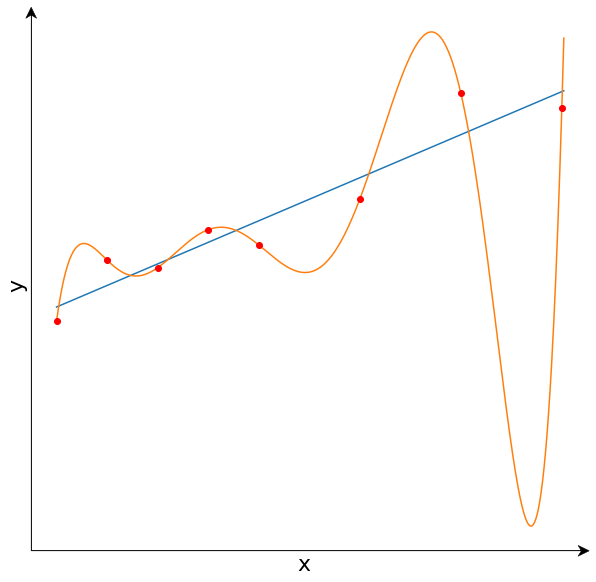
\includegraphics[scale=0.35]{images/overfit.png}
		\centering
		\caption{A toy overfit example. Red points represent two-dimensional linear data with some noise. While linear model explains the data not perfectly, it achieves a good generalization. The more powerful seventh degree polynomial model fitted the data ideally, but failed to generalize. }
	\end{figure}
	
	
	To detect the overfitting, one needs to test a model over data not included into the training set. Thus, not all data are being fed into the model during training, but some part is being left untouched until it comes to the estimator performance evaluation. This piece of data is often referred as a \textbf{test set}.
	
	\begin{figure}[h]
		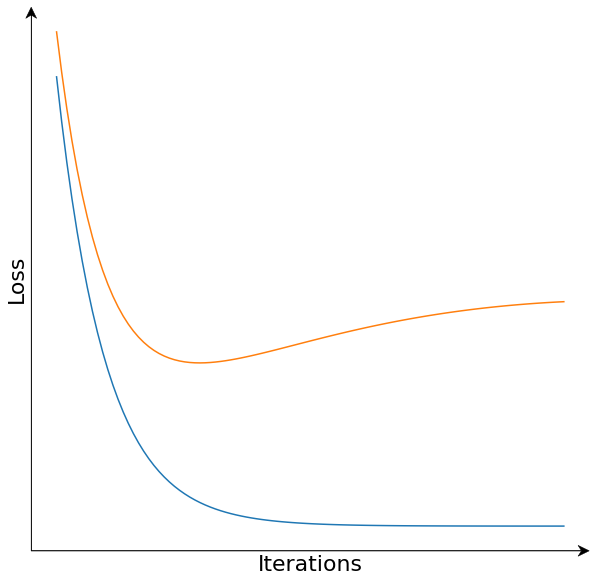
\includegraphics[scale=0.35]{images/generic_loss_graph.png}
		\centering
		\caption{Typical loss-by-iteration training graph. The blue graph represents training loss, which monotonically (in practice with some oscillation) decreases the more training iterations the model passed. The yellow graph represents validation loss, which starts to grow at the same time the model starts to overfit}
	\end{figure}
	
	Overfitting is a frequent situation when powerful models, such as artificial neural nets, are being used. These models may represent a very large set of different functions, including more complex than is necessary to describe the distribution from which the training set was drawn. The problem is in dense relation with the Occam's Razor, and an overfitting occured implies violation of the principle\cite{overfitting}---the model tries to describe the data by inferring patterns which don't exist.
	
	To combat overfitting, variety of methods is being applied:
	\begin{itemize}
		\item \textbf{Gathering more data.} More samples \textit{from the same distribution} means that during training the model will see more diverse and densely located data points, and will be less prone to memorizing instead of pattern extraction. One should pay attention to the data quality while collecting them: low-quality and noisy data may \textit{decrease} the model performance.
		
		\item \textbf{Usage of a simpler model.} It's possible to design a model powerful enough to explain data, but too weak to yield an overcomplicated function, since noise's pattern is random and therefore more complex.
		
		\item \textbf{Regularization.} Regularization is a process of adding additional constraints to the model. This technique is densely related to the previous point---regularized model's representative power is being limited to fit the data but not the noise.
		
		Model weight norm is usually being penalized to produce smoother functions; artificial neural nets may be regularized by zeroing output of a random neuron during training (so-called \textit{dropout}). Further regularization techniques also exist.
		
		\item \textbf{Data augmentation.} Data augmentation is a technique of an artificial samples number increasing without collecting more data. This involves transforming a sample without changing its semantic. A typical example is an image mirroring and rotation: if the task is to classify a cat photo as "Cat", the mirrored or rotated image still will contain the cat on it and may be appended to the training set under the same label.
		
	\end{itemize}
	
	It's worth to mention that \textbf{underfitting} also may occur when the model:
	\begin{itemize}
		\item Wasn't trained enough and needs more training iterations to fit the data
		\item \textit{Too weak} to fit the data
	\end{itemize}
	
	The second case may be illustrated by fitting the quadratic data with linear regression model. Model weakness usually appears as similar, unsatisfying and not improving performance on both training and test data. The solution is straightforward: more complex model.
	
	\subsection{Models and Hyperparameter Tuning}
	
	Machine learning \textbf{model} is a parameterized function used to approximate and generalize the underlying data. This function may be represented by a mathematical function (linear regression), set of rules (decision trees) or more complex methematical structure (neural networks). The model itself may represent multiple specific functions depending on its parameters, and the training process is being run to automatically pick them.
	
	But there are values responsible to the \textit{shape} of model, such as a polynomial degree in polynomial regression, tree depth in decision trees or an entire neural network architecture. These values cannot be learned since they have to be defined before the model instantiation, and should be picked by a machine learning specialist. These values are called \textbf{hyperparameters} and the process of picking the right hyperparameter value is called \textit{tuning}. Tuning stands on analysing the model performance on unseen data after training.
	
	Hyperparameters cannot be tuned on the same data the model performance is being estimated on. By picking the best hyperparameter after testing it on a certain data set, one adapts the model to this specific piece of data, and the model performance on it will be biased towards the better result. Thus, one has to tune hyperparameter on a \textbf{validation} data set disjoint from training and test sets.
	
	Summary:
	\begin{itemize}
		\item On the \textbf{training} set the model is being trained
		\item By performance on the \textbf{validation} set the best model is being chosen
		\item The model performance on the \textbf{test} set is an unbiased estimation of its performance in practice
	\end{itemize}
	
	\section{Deep Learning}
	
	\subsection{What is Deep Learning?}
	
	\textbf{Deep learning} is a subset of machine learning relying on deep artificial neural networks (ANN) application. The word "deep" refers to the large number of hidden layers of the neural networks being used.
	
	Deep Learning is notably different from the rest of machine learning methods, primarily due to the unique ANN capabilities. The key differences are:
	\begin{itemize}
		\item \textbf{No feature engineering required.} Classic ML algorithms heavily rely on the initial process of constructing more representative features from the raw data. This approach is problem-specific and often requires an expertise in a related domain. One of the most important (if not the most one) of the ANN advantages is a capability to infer high-level features by themselves, simplifying the data preparation and letting the ML specialist to approach a problem without a domain-specific expertise.
		
		\item \textbf{DL approach can produce end-to-end solutions.} Classic ML approach requires a problem breakdown to several subtasks, which are then being individually approached with different models and a manual feature engineering. Deep Learning allows to produce a monolith model able to produce output directly after being fed with data. This not only simplifies the model development, but also ensures that the model is being trained as a whole, forcing its components to adapt to each other.
		
		\item \textbf{ANNs often can be transferred to solve similar problem.} An already trained ANN can be used as a baseline for an another task solution. By partial or full re-training this ANN on a new data the better and faster result may be achieved. One of the most common applications of the \textit{transfer leraning} is an image recognition\cite{how_transferable}.
		
		\item \textbf{ANNs often require huge amount of data for training\dots}
		This disadvantage is related primarily to classification/regression ANNs, since the only accompanying information they get with a sample during training is a single value. If the model gets an image with a "Cat" label, it has to infer by itself what is needed to classify this image as "Cat". Since most state-of-art deep learning models got millions of parameters, this requires proportional data amount to not overfit.
		
		\item \textbf{\dots but sometimes they not.} At the same time, several ANN architectures (for semantic segmentation, object detection, \dots) during training recieve a ground truth map instad of a label. This map contains a target value \textit{for an every pixel}. Such amount of related information may be enough to train a model from scratch on tens of images, like the well-known U-Net\cite{unet}.
		
		\item \textbf{ANN training requires a lot of computational power.} ANNs are based on numerous matrix multiplications, which are memory-hungry and require specialized hardware such as GPU or TPU for speeding up. This disadvantage limits ANN combination with several time-consuming techniques like cross-validation or ensembling.
		
		\item \textbf{ANNs are hard to interpret.} Another major advantage of conventional ML approach and the reason why it still dominates in several sectors. While it's pretty easy to interpret and visualize linear regression models or decision trees, ANN makes its decisions through numerous matrix multiplications which are hard to depict graphically and explain in human terms.
		
		Neural network interpretability is a wide field for research. There is a certain progress\cite{simonyan2013deep}\cite{fan2020interpretability}, but the problem hasn't yet been solved exhaustively.
	\end{itemize} 
	
	\subsection{Artificial Neural Networks}
	
	\textbf{Artificial Neural Network (ANN)}, or a \textbf{connectionist system}, is a mathematical model and its implementation inspired by the biological neural networks. The ANN building principles were initially formalized by McCulloch and Pitts\cite{McCulloch43}, while the Hebbian theory\cite{hebb-organization-of-behavior-1949} became the basis of the ANN learning. Initially emerged as attempts to simulate the mechanisms of the brain, ANNs evolved to one of the most powerful tools in data analysis nowadays.
	
	\subsubsection{Artificial Neuron as a Model}
	The primary ANN building block is an artificial neuron. Its prototype is a biological neuron, which receives input signals via its \textit{dendrites} and transmits its output through the single \textit{axon}. The axon later branches and connects to another neurons' dendrites via \textit{synapses}. Depending on the synaptic strength and its direction (excitory or inhibitory), input signal received through a certain synapse may increase or decrease the \textit{postsynaptic potential}. If this potential exceeds a certain threshold, the neuron \textit{fires} and sends an output signal through its axon. The information the neuron transmits is being encoded into the neuron's \textit{fire rate}.
	
	\begin{figure}[h]
		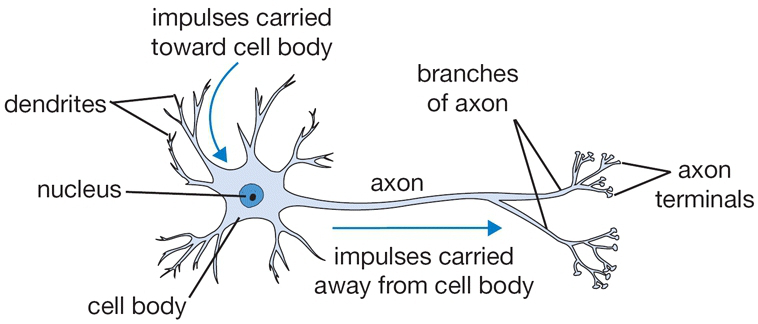
\includegraphics[width=10cm]{images/neuron.png}
		\noindent\rule{8cm}{0.4pt}
		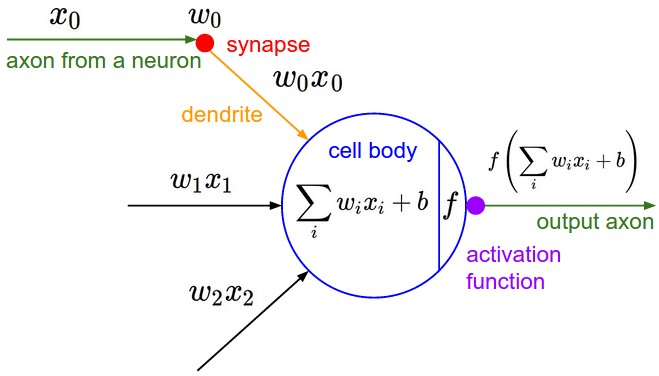
\includegraphics[width=10cm]{images/neuron_model.jpeg}
		\centering
		\caption{A comparison of a biological neuron (top) and its matematical model (bottom). Pictures taken from the CS231n course\cite{cs231n}.}
	\end{figure}
	
	The artificial neuron models that process by accepting several numeric signals (e.g. $x_i$) which interact with corresponding synapses (e.g. $w_i$) multiplicatively (e.g. $x_iw_i$). The synapse connection strength and direction correspond with the $w_i$ (or $i$\textsuperscript{th} \textbf{weight}) absolute value and sign respectively, and define how one neuron influences another. The postsynaptic potential then is a weighted sum of input signals. This potential is later being summed with the \textbf{bias} term modeling the fire threshold, and the fire rate is being modeled by the non-linear \textbf{activation function}. The main assumption there is that neuron's weights are learnable, same as synaptic strengths between biological neurons.
	
	The artificial neuron output formula may be written as:
	
	\[y = \sigma(x^Tw)\]
	where $y$ is the neuron's output, $\sigma$ is an activation function, $w$ is a neuron's weight vector and $x$ is an input vector with additionally defined $x_0$ as 1:
	\[x = (1, x_1, x_2,\dots)\]
	which allows to encode the bias as $w_0$.
	
	It's important to mention that this model of a biological neuron is very coarse. Both axons and dendrites perform non-linear computations over signals instead of simple transmission; synaptic connections are not linear but complex and dynamic; the fire rate encoding without taking timing into account is also a rough approximation. Specifically this mathematical model is not intended to model the biological neuron in details, but to represent a computing unit suitable for building both expressive and computationally efficient models. Keeping it in mind, further in this work an artificial neuron will be referred simply as a neuron.
	
	\subsubsection{Feedforward Neural Networks}
	A single neuron itself may represent a binary linear classifier. By using a Heaviside step function defined as:
	
	\[
	\mathcal{H}(x) = 
	\begin{cases}
	0, & \text{if}\ x<0 \\
	1, & \text{if}\ x \geq 0
	\end{cases}
	\]
	as an activation, a neuron can split an input space with an affine hyperplane and thus with proper weights perfectly classify linearly separable data.
	
	Nonetheless, most of data one can meet in practice are not linearly separable. To introduce more complex functions rather than linear ones, neurons are being arranged so that output of several neurons propagates to other neurons. There is a wide variety of different network arrangements\cite{nn_zoo}, but one of the most common and simple is a \textbf{feedforward neural network (FFNN)}.
	
	\begin{figure}[h]
		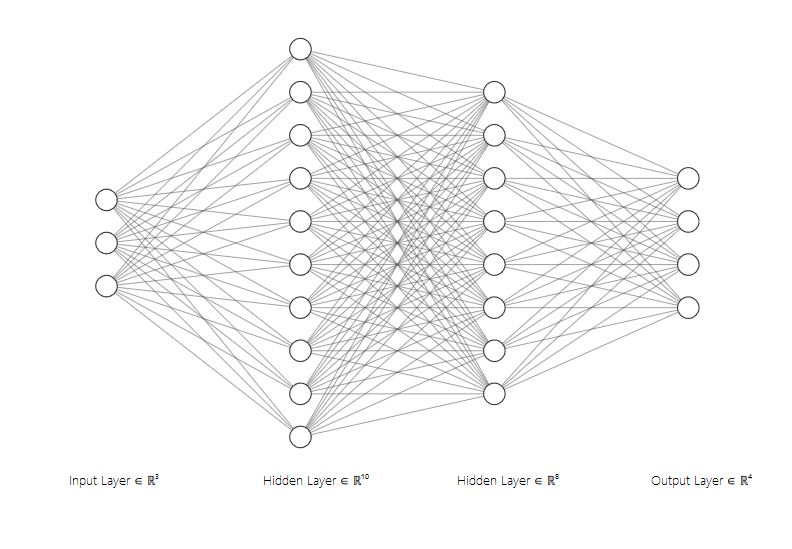
\includegraphics[width=\textwidth]{images/ffnn.png}
		\caption{Example of a FFNN with two hidden layers. Visualized using NN-SVG\cite{nn-svg}.}
	\end{figure}
	
	FFNN consists of neurons arranged into \textbf{layers}. Layer is a tuple of neurons, each of which gets the same input vector as others. In respond to the input, the layer's neurons produce their own outputs which are then being composed into the layer's output vector and being sent to the next layer. The information flows from the previous layer to the next one without cycles until reaches the output layer. FFNN layers may be split into:
	\begin{itemize}
		\item Single \textbf{input} layer. Each element of the input layer is not a neuron but an input vector value being propagated to the all neurons of the next layer.
		\item Several \textbf{hidden} layers. These get an input from the previous layer and send their output to the next one
		\item Single \textbf{output} layer. Output of this layer is being considered as a neural network decision. It may contain a single neuron with an identity activation function for regression or $n$ neurons with linear or softmax\cite{softmax} activation function for $n$-ary classification.
	\end{itemize}
	
	Let $d(i)$ be the dimensionality of the $i$\textsuperscript{th} layer output and let $d(0)$ be the neural network's input dimensionality. The $i$\textsuperscript{th} layer then may be defined as a function $l_i : \mathbb{R}^{d(i-1)} \mapsto \mathbb{R}^{d(i)}$:
	
	\[l_i(y) = \sigma_i(y^TW_i)\]
	where $y$ is the layer's input, $\sigma_i$ is the layer's activation function and $W_i$ is the layer's weight matrix with $d(i)$ columns and $d(i-1)$ rows. $n$\textsuperscript{th} column there corresponds to the weight vector of the $n$\textsuperscript{th} neuron.
	
	Note that the $y$ is being one-padded before multiplication, same as in the neuron formula defined before:
	\[y = (1, y_1, y_2, \dots)\]
	The first row of $W_i$ therefore corresponds to the biases of certain neurons.
	
	Using this definition, the $n$-layer feedforward neural network output may be defined as a composed function $\mathcal{F} : R^{d(0)} \mapsto R^{d(n)}$:
	\[\mathcal{F}(x) = l_n \circ l_{n-1} \circ \dots \circ l_2 \circ l_1\]
	The non-linear activation function is crucial. Without it, the whole neural network could be expressed by the single matrix multiplication, and wouldn't be more powerful than linear classifier. Thanks to the non-linearity and layered structure, FFNN with a single hidden layer represents a universal approximator\cite{universal_approx_wiki}\cite[Chapter~4]{nndl_universal_approx}.
	
	\subsubsection{Backpropagation}
	
	The most widely used learning algorithm for neural networks is the \textbf{backpropagation}, or \textbf{backprop}. The words "backpropagation" and "gradient descent" can be very often met together, and their meanings mostly intersect with each other. Basically, backprop may be defined as a neural network variation of the gradient descent and a way to compute the gradient efficiently by applying the chain rule\cite{chain_rule}.
	
	\begin{figure}[h]
		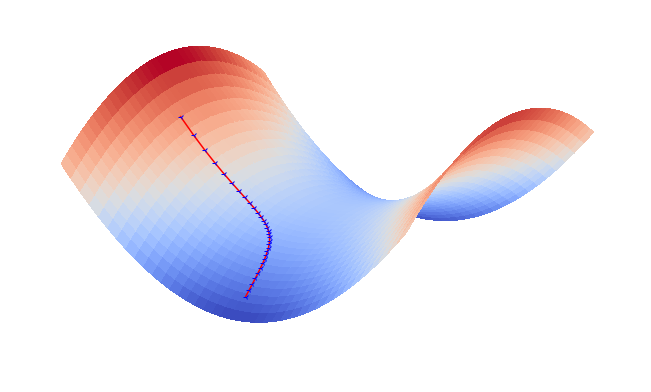
\includegraphics[width=\textwidth]{images/grad.png}
		\caption{Gradient descent visualization. The two-dimensional variable space represents model parameter values; $z$-axis is the training loss function value. Starting at some point (pre-trained or randomly initialized), the training algorithm computes the gradient at this point, multiplies it by the learning rate and subtracts it, yielding the new point with the lower loss function value. In case of a real ANN, a variable space is being million-dimensional with a non-trivial relief.}
	\end{figure}
	
	The method basis is to iteratively compute the loss function gradient with respect to the model's weights, and use it to perform the weight update. The iteration step may be written as:
	
	\[W^{(i+1)} = W^{(i)} - \gamma \nabla \mathcal{L}(W^{(i)},\; \mathcal{X})\]
	where:
	\begin{itemize}
		\item $W^{(i+1)}$ is the vector of all model weights at the $(i+1)$\textsuperscript{th} step
		\item $\nabla \mathcal{L}(W^{(i)},\; \mathcal{X})$ is the gradient of the mean loss function value over the dataset $\mathcal{X}$ with the model weights $W^{(i)}$ computed with respect to $W^{(i)}$. The term is negative since the gradient points to the steepest \textit{growth} direction; during training the aim is the loss minimizing instead.
		\item $\gamma$ is the \textbf{learning rate (LR)} parameter responsible for the step size
	\end{itemize}
	
	The learning rate is very important. A too high value won't let the model approach the minimum, forcing it to "bounce" near it; it also may "kill" neurons using ReLU as an activation function, which will be discussed later. A too low value is impractical and will inefficiently consume computing resources. The common practice is an initial LR value in range $10^{-4}$---$10^{-5}$, which is varied through the training.
	
	\begin{figure}[h]
		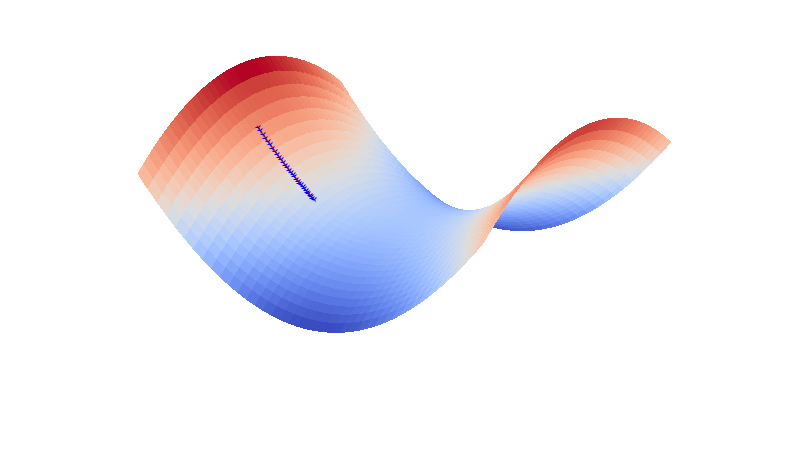
\includegraphics[width=\textwidth]{images/low_lr.png}
		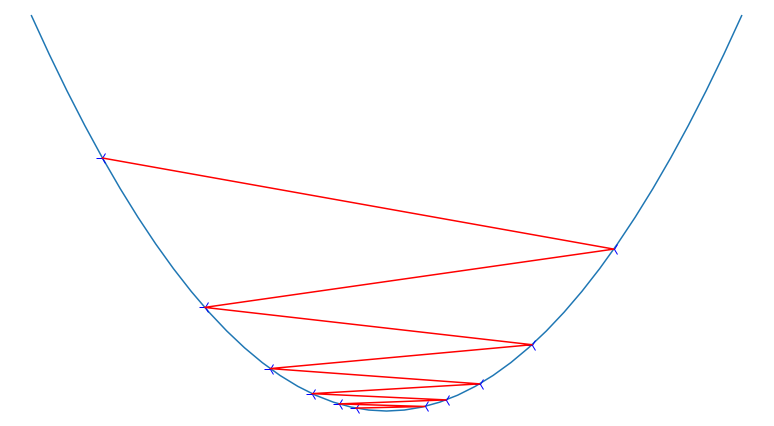
\includegraphics[width=\textwidth]{images/high_lr.png}
		\centering
		\caption{Low and high learning rate toy examples. A too low LR value (above) slows the training down and sometimes may lead to being stuck in a shallow local minimum (not illustrated). A too high LR value (below) leads to several another problems, one of which is overshooting loss minima.}
	\end{figure}
	
	To compute the gradient, the chain rule\cite{chain_rule} is being employed. It allows to compute gradients of earlier layers re-using the previously computed gradients of later layers. To describe and implement the information flow inside the ANN, the \textbf{computational graph} conception is being used.
	
	\begin{figure}
		\centering
		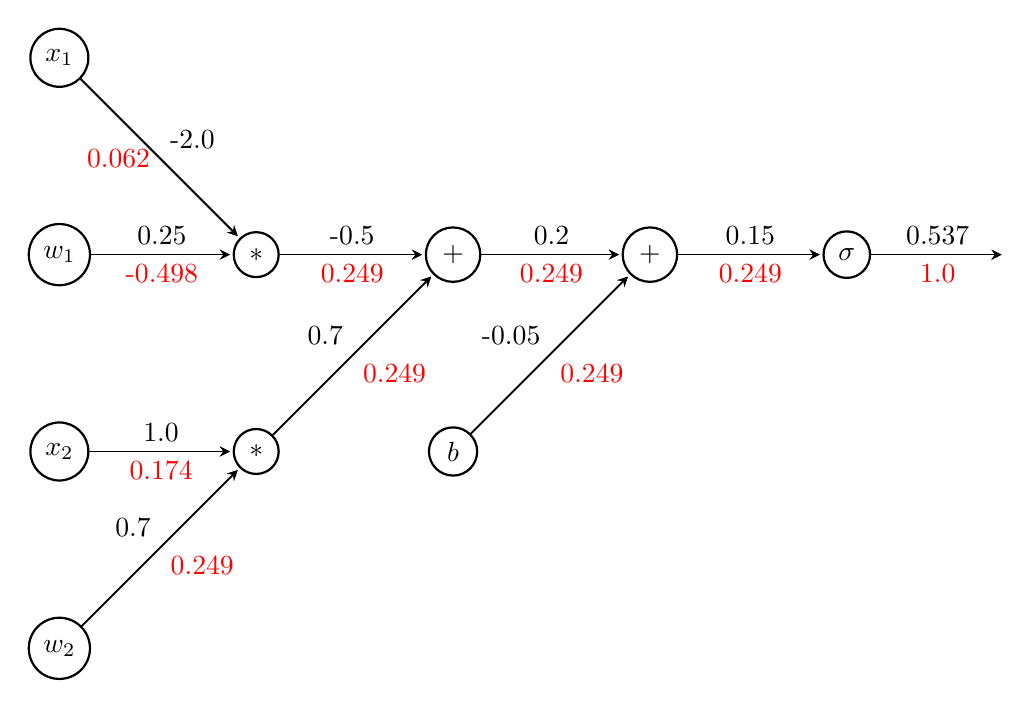
\begin{tikzpicture}[
		> = stealth, % arrow head style
		shorten > = 1pt, % don't touch arrow head to node
		auto,
		node distance = 2.5cm, % distance between nodes
		semithick % line style
		]
		
		\tikzstyle{every state}=[
		draw = black,
		thick,
		fill = white,
		minimum size = 4mm
		]
		
		\node[state] (inp_x1) {$x_1$};
		\node[state] (w1) [below of=inp_x1] {$w_1$};
		\node[state] (inp_x2) [below of=w1] {$x_2$};
		\node[state] (w2) [below of=inp_x2] {$w_2$};
		\node[state] (mul_1) [right of=w1] {$*$};
		\node[state] (b) [below of=w2][right of=mul_1] {$b$};
		\node[state] (mul_2) [right of=inp_x2] {$*$};
		\node[state] (sum_1) [right of=mul_1] {$+$};
		\node[state] (sum_2) [right of=sum_1] {$+$};
		\node[state] (sigmoid) [right of=sum_2] {$\sigma$};
		
		\path[->] (inp_x1) edge node {-2.0} (mul_1);
		\path[->] (w1) edge node {0.25} (mul_1);
		\path[->] (inp_x2) edge node {1.0} (mul_2);
		\path[->] (w2) edge node {0.7} (mul_2);
		\path[->] (mul_1) edge node {-0.5} (sum_1);
		\path[->] (mul_2) edge node {0.7} (sum_1);
		\path[->] (sum_1) edge node {0.2} (sum_2);
		\path[->] (b) edge node {-0.05} (sum_2);
		\path[->] (sum_2) edge node {0.15} (sigmoid);
		%\path[->] (sigmoid) edge node {0.537} (out);
		\draw [->] (sigmoid) edge node {0.537} ++ (2,0);
		
		\path[->] (inp_x1) edge node[left] {\color{red}0.062} (mul_1);
		\path[->] (w1) edge node[below] {\color{red}-0.498} (mul_1);
		\path[->] (inp_x2) edge node[below] {\color{red}0.174} (mul_2);
		\path[->] (w2) edge node[below right] {\color{red}0.249} (mul_2);
		\path[->] (mul_1) edge node[below] {\color{red}0.249} (sum_1);
		\path[->] (mul_2) edge node[below right] {\color{red}0.249} (sum_1);
		\path[->] (sum_1) edge node[below] {\color{red}0.249} (sum_2);
		\path[->] (b) edge node[below right] {\color{red}0.249} (sum_2);
		\path[->] (sum_2) edge node[below] {\color{red}0.249} (sigmoid);
		\draw [->] (sigmoid) edge node[below] {\color{red}1.0} ++ (2,0);
		\end{tikzpicture}
		\caption{Example computational graph of a single neuron with the sigmoid activation function. On the forward pass the neuron receives inputs and computes an output. During the backward pass the differentials of all nodes are being numerically computed using the forward pass values and gradients of their nodes-successors. The computational graph receives an initial gradient value of 1.0, since this is the derivative of the computational graph output by the computational graph's last node output (which are the same).}
	\end{figure}
	
	Computational graph is a directed graph representing a composed function. A graph node is a differentiable mathematical operation, while node inputs are values---produced by previous nodes or input constants. Further in the chapter it will be assumed that computational graphs are acyclic---all considered architectures don't contain cycles.
	
	By plugging in the input values with weights and traversing through the graph along the connection directions, the output value is being computed. This is called the \textbf{forward pass}.
	
	During the model training, it's needed to compute the \textit{global} differential of a certain model weight---the differential of a whole model output with respect to this weight. The computational graph conception allows to break this task down to computing several \textit{local} gradients and multiplying them with each other:
	
	\[y(x) = f(g(x)) \implies \frac{\partial y}{\partial x} = \frac{\partial f}{\partial g} \frac{\partial g}{\partial x}\]
	
	According to the computational graph conception, the gradient computing may be interpreted as traversing the computational graph \textit{backwards}:
	\begin{enumerate}
		\item The graph node receives through its output edge the gradient of the whole model with respect to this node value. If there are more than one gradients received, they are being summed.
		\item The local gradients (of this node output with respect to each of this node inputs) are being computed.
		\item Each local gradient is being multiplied by the gradient received by node to get the \textit{global} gradient.
		\item The obtained gradients are being sent further, towards the earlier model layers.
	\end{enumerate}
	
	\begin{figure}[h]
		\centering
		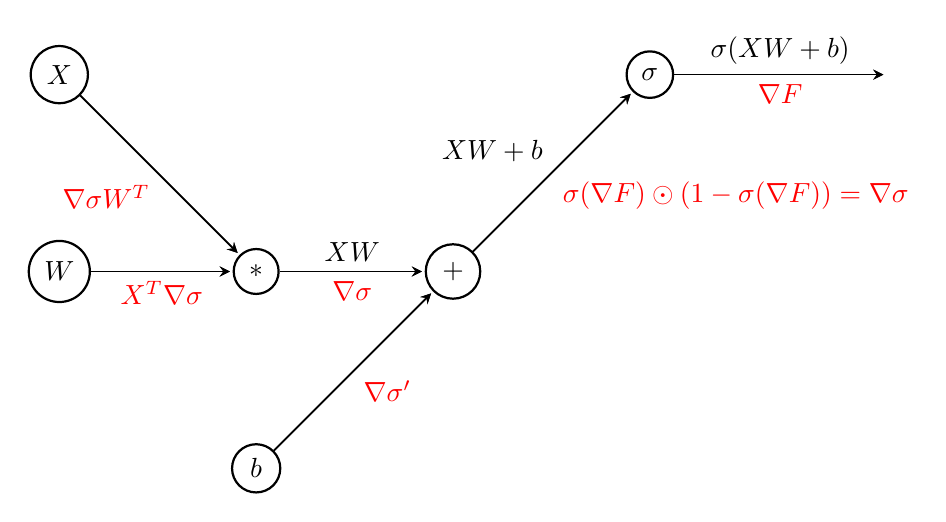
\begin{tikzpicture}[
		> = stealth, % arrow head style
		shorten > = 1pt, % don't touch arrow head to node
		auto,
		node distance = 2.5cm, % distance between nodes
		semithick % line style
		]
		
		\tikzstyle{every state}=[
		draw = black,
		thick,
		fill = white,
		minimum size = 4mm
		]
		
		\node[state] (X) {$X$};
		\node[state] (W) [below of=X] {$W$};
		\node[state] (mul) [right of=W] {$*$};
		\node[state] (b) [below of=mul] {$b$};
		\node[state] (sum) [right of=mul] {$+$};
		\node[state] (sigmoid) [right of=sum][above of=sum] {$\sigma$};
		
		\path[->] (X) edge node {} (mul);
		\path[->] (W) edge node {} (mul);
		\path[->] (mul) edge node {$XW$} (sum);
		\path[->] (b) edge node {} (sum);
		\path[->] (sum) edge node {$XW+b$} (sigmoid);
		\draw [->] (sigmoid) edge node {$\sigma({XW+b})$} ++ (3,0);
		
		\path[->] (X) edge node[below left] {$\color{red}\nabla \sigma W^T$} (mul);
		\path[->] (W) edge node[below] {$\color{red}X^T \nabla \sigma $} (mul);
		\path[->] (mul) edge node[below] {$\color{red}\nabla \sigma$} (sum);
		\path[->] (b) edge node[below right] {$\color{red}\nabla \sigma '$} (sum);
		\path[->] (sum) edge node[below right] {$\color{red} \sigma(\nabla F) \odot (1 - \sigma(\nabla F)) = \nabla \sigma$} (sigmoid);
		\draw [->] (sigmoid) edge node[below] {$\color{red}\nabla F$} ++ (3,0);
		
		
		\end{tikzpicture}
		\caption{Matrix form of the FFNN layer computational graph with the sigmoid activation function, where $\nabla F$ is a global gradient by the layer's output. The "$+$" node is defined as "add the $b$ vector to the every $XW$ row". $\nabla \sigma '$ therefore means mean value of $\nabla \sigma$ rows---a sum of $b$ gradients scaled down to be not dependent on the input batch size.}
	\end{figure}
	
	During training, the initial gradient value received by the neural net will be the gradient of the mean loss function value over the training dataset with respect to the neural net output. The word "gradient" is being used in this subsection often to mention that practical implementations operate with tensors, not individual values themselves.
	
	In practice, due to memory issues its impossible to feed the whole dataset into the neural network at once. Instead, data are being fed by \textit{batches} randomly sampled from the dataset. This variation of the algorithm is called \textbf{Stochastic Gradient Descent (SGD)}. "Stochastic" means that that batches are randomly selected and meant to approximate the input data distribution.
	
	\subsubsection{Activation Functions}
	
	Since the neural network is being trained by computing its gradient, it's crucial that the \textbf{activation function must be differentiable}. Elder models used tanh and sigmoid functions, which are differentiable for all arguments and their derivatives for any specific arguments may be computed using their values. Minor drawback of a sigmoid function is that its output is not zero-centered which negatively influences the model training, but the major issue why sigmoind and tanh are not being used widely is that they \textbf{saturate}.
	
	\begin{figure}[h]
		\centering
		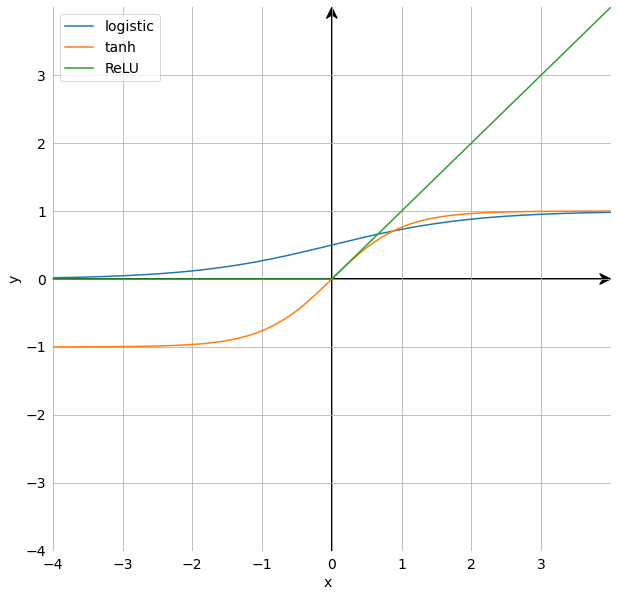
\includegraphics[scale=0.35]{images/activations.png}
		\caption{Three common activation functions illustrated. While logistic sigmoid and $\tanh$ functions saturate in both directions, ReLU saturates in only one. ReLU is also easier to compute both during forward and backward pass.}
	\end{figure}
	
	With growing argument's absolute value, the derivative of tanh and sigmoid quickly decreases to small values. If the neuron using such function produces large enough postsynaptic potential, the activation function becomes saturated and the gradient flow through this neuron is being multiplied by the value close to zero. As seen on the equations above, layers interact with each other multiplicatively, and several saturated activation functions may paralyse training.
	
	To get around this, the \textbf{Rectified Linear Unit (ReLU)}\cite{sparse_rectifier} and its variations are being used by the most state-of-art models. ReLU value is defined as
	\[\text{ReLU}(x) = \max(0, x)\]
	
	It's not differentiable for $x = 0$, the derivative at this point may be defined as 0 or $x$. Its output is not zero-centered also. But it doesn't suffer from saturating and is computationally more efficient than sigmoid functions.
	
	ReLU's major drawback is that it introduces the \textbf{dying neurons} problem. With a too high learning rate, the neuron may get such a weight update that it will never fire again on the same data. The gradient flow through this neuron is being zero, and it will not get a new weight update. Lower learning rates help to avoid it, while some ReLU variations\cite{wiki_relu}, such as leaky or exponential ReLU, don't suffer this problem.
	
	\subsubsection{Dropout}
	
	Earlier in this chapter it was mentioned that ANNs are easy to overfit. While another methods include weight norm constraints and reducing the number of free parameters\cite{lecun_generalization}, Siravastava et al.\cite{dropout} introduced another technique of achieving a better ANN generalization---a so-called \textbf{Dropout}.
	
	Overfitting of an ANN is often being shown as a high absolute value of certain weights. This means that the layer actually uses only small subset of its inputs to produce an output. Once a certain feature is not present in an input sample, the neural network makes a wrong decision.
	
	To combat this and force the neural network use more of its inputs, Siravastava et al. proposed to zero random values of a layer input during training with a certain chance $p$. By doing this, the neural network is being forced to take into account a possible absence of a certain feature and rely on more of its inputs rather than on limited subset.
	
	\begin{figure}[h]
		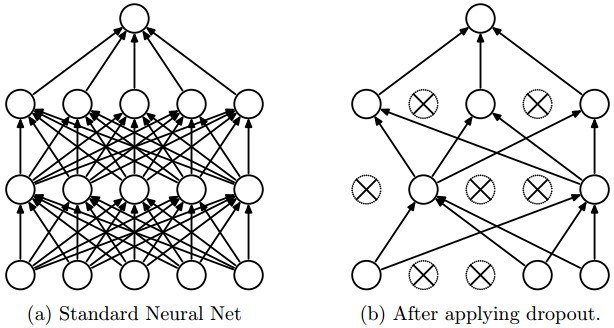
\includegraphics[width=\textwidth]{images/dropout.jpeg}
		\caption{Illustration taken from the Dropout paper\cite{dropout}. During training time only fraction of ANN connections is being subsampled and properly rescaled. During test time neurons see all their inputs. One of the proposed Dropout interpretations says, that during the test time different models sampled from the original one are being averaged.}
	\end{figure}
	
	This technique has got a lot in common with the $L^2$ regularization (which will be discussed later)---both methods work primarily against high weight norms, and produce more diffuse weight vectors.
	
	The important detail of a dropout realization is that once the dropout is being applied, the input is being multiplied by $1/(1-p)$. This is needed to keep the neuron outputs during train (when dropout is being applied) and test/inference (when all inputs are in place) time at the same scale.
	
	In terms of mathematics, dropout is a Hadamard product of an input with a dropout matrix. This matrix has a zero cell with a chance of $p$ or a $1/(1-p)$ cell otherwise. Therefore, during backpropagation a local gradient will be a dropout matrix applied during the forward pass.
	
	\subsection{Convolutional Neural Networks}
	
	\textbf{Convolutional Neural Network (CNN)} is a special ANN architecture proposed by Yann LeCun in 1989\cite{LeCunBoserDenkerEtAl89}. While FFNNs originated as simulations of the brain mechanisms in common, CNNs borrow a lot from the visual cortex\cite{hubel1962receptive}. Thanks to their properties, they became one of the most effective models for visual recognition, and still keep the position of the state-of-art model family.
	
	\subsubsection{Motivation}
	
	While FFNNs had shown themselves as flexible and powerful models, they have their own drawbacks which don't let to directly apply them in certain domains:
	\begin{itemize}
		\item \textbf{FFNNs poorly scale for images.} FFNN's first hidden layer accepting a $128 \times 128 \times 3$ image would have 49152 weights per neuron, and a single bias. A typical FFNN has got several layers of hundreds and thousands of neurons, and a total parameter count for image recognition tasks can quickly grow out of limits.
		\item \textbf{FFNNs don't take spatial information into account.} The only interaction input value participates in layer is a weighted sum with all another input values---no input correlations are being tracked, while an image semantics mostly depends on such correlations. FFNN is also not invariant to the image shift---the feature learned from the one image may be not detected on the shifted image, even if shifted image semantics is the same.
	\end{itemize}
	
	\subsubsection{Convolutional Layer}
	
	To overcome this issues, CNN introduces several new building blocks for working with a spatially-arranged information.
	
	The main building block of a CNN is a \textbf{convolutional layer}, or ConvLayer. Instead of a weight vector, its neuron uses a learnable two- or three-dimensional \textbf{filter}, or \textbf{kernel}. While one-dimensional ConvLayers are also being used (in natural language processing, for example), further in this section it will be assumed that convolutional layer operates with two spatial dimensions and a single depth dimension.
	
	Convolutional layer produces its output by performing a discrete convolution operation of its kernels over an input image. Kernels are 3D (assuming a multi-channel image as input) tensors, being typically small along spatial dimensions ($3 \times 3$, $5 \times 5$ or $7 \times 7$) but having the same depth as an input image. Convolution of a kernel with an input image may be defined as "sliding" the filter across the width and height of the image and computing a dot product of the kernel weights and image values.
	
	The result of the convolution is a two-dimensional \textbf{feature map}, which may be interpreted as a distribution of some distinct feature (being represented by the filter) over the image. Since ConvLayer typically contains tens or hundreds of kernels (mostly powers of two in range 32-512), an output of the convolutional layer is also an image with the depth equal to the kernel count.
	
	\noindent
	Such a layer organization brings several benefits:
	\begin{itemize}
		\item \textbf{Parameter re-use}. A ConvLayer parameter count is much lower due to low filter sizes across spatial dimensions. This is possible thanks to the assumption that a certain feature is not tied spatially to a certain location on an image.
		\item \textbf{Neuron activation is translation invariant}. Since a kernel is being applied to a whole image region-by-region, the feature it represents will be detected on the shifted image too---it will just appear at another place of the output map.
		\item \textbf{ConvLayer may accept images of different shapes}. The only difference is a number of dot product computations and an output spatial size.
		\item \textbf{Natural semantics}. Applied researches\cite{zfnet} show that each filter represents a certain feature which (primarily for first ConvLayers) may be visualized. Convolution outputs a feature map, which may be interpreted as a spatial distribution of a certain feature across the image, and may be also easily visualized and used for the neural network behavior study.
	\end{itemize}
	
	\begin{figure}[h]
		\centering
		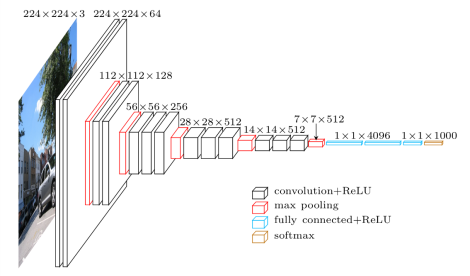
\includegraphics[scale=0.66]{images/vgg16.png}
		\caption{VGG16\cite{vgg} architecture illustrated. Taking a $224 \times 224 \times 3$ image as input, by an alternating application of $3 \times 3$ filters, non-linearities and MaxPools the model gradually shrinks the data spatially, adding more and more of a high-level information and stacking it along the depth axis. The later layers operate a high-level information, relying on features extracted by previous layers and capturing a significant spatial context.}
	\end{figure}
	
	In addition to the filter count, convolutional layer has got several another important hyperparameters:
	\begin{itemize}
		\item \textbf{Filter size}. Spatial kernel size defines a filter's \textbf{receptive field}---a region of an image the kernel convolves at the same time. Before the VGG-Net\cite{vgg} was introduced, it was common to have $7 \times 7$\cite{zfnet} or even $11 \times 11$\cite{alexnet} filters at first ConvLayers. VGG-Net later showed that several combined filters of lower size introduce both more flexibility and lesser parameter count at the cost of additional layers. Nowadays, most of ConvNets still keep homogenous $3 \times 3$ filter pattern across the whole model, except first layers where larger kernel sizes are often being present.
		\item \textbf{Padding}. Since the convolution operation changes input's spatial size (except layers with $1 \times 1$ kernels), padding is often being employed to keep it constant. Padding prevents maps from shrinking after passing multiple convolutions, and simplifies a model design by eliminating the need to re-compute the output size after each convolution.
		\item \textbf{Stride}. Stride is a step size when moving a filter during convolution. Using strides larger than one aggressively reduces an output map size, and is mostly being used at first ConvLayers for the dimensionality reduction.
	\end{itemize}
	
	\subsubsection{Another New Building Blocks}
	
	\begin{figure}[h]
		\centering
		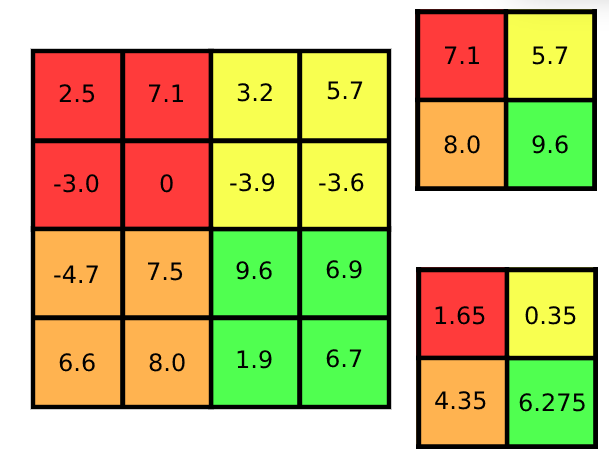
\includegraphics[scale=0.5]{images/pool.png}
		\caption{Pooling layer illustrated. The $4 \times 4$ grid represents an image, while $2 \times 2$ grids represent Max (top) and Average (bottom) pooling operation results. Precisely, max/average $2 \times 2$ pooling with stride 2.}
	\end{figure}
	
	Convolutional layer is not the only spatial-specific layer being used in ConvNets.
	
	\textbf{Pooling layers} are used to spatially reduce an image. The most common are Max and Average Pooling layers, which divide an image spatially into cells of a certain size (typically $2 \times 2$ or $3 \times 3$) and take a maximum or a mean value respectively. The cells may be disjoint (stride is equal or larger than a cell size), or may have an intersection (e.g. $3 \times 3$ pooling with stride 2).
	
	It's common to place a pooling layer after several convolutions---pooling layer rejects weak activations (for Max Pool) or combines them (for Average Pool), and a spatial reduction of a feature map increases a receptive field of preceding convolutional layers.
	
	\textbf{Spatial Dropout} is a modification of a Dropout technique for using with 2D feature maps. Original Dropout works poorly on regularizing models working with correlated values---zeroing a random input won't affect it's neighbours, and they still will activate the filter. The Spatial Dropout solves this by zeroing an entire feature map instead.
	
	This is similar to the original Dropout working mechanism in FFNN---zeroing a random input of FFNN layer may be interpreted as excluding a certain feature from the input. Sice in CNNs, instead of distinct values, features are being represented by feature maps, to exclude a certain feature from an input it's needed to exclude a whole feature map.
	
	\subsubsection{Implementation and Backprop}
	Convolution operation is computationally heavy. To accelerate it, it is usually being implemented as a matrix multiplication by using so-called \textbf{im2col} or \textbf{im2row} operations.
	
	\begin{figure}[h]
		\centering
		
		$\begin{bmatrix}
		w_{11} & w_{12}\\
		w_{21} & w_{22}\\
		\end{bmatrix} \longrightarrow \begin{bmatrix}
		w_{11} & w_{12} & w_{21} & w_{22} 
		\end{bmatrix} = W$
		$\begin{bmatrix}
		0 & 0 & 0 & 0\\
		0 & x_{11} & x_{12} & 0\\
		0 & x_{21} & x_{22} & 0\\
		0 & 0 & 0 & 0\\
		
	\end{bmatrix} \longrightarrow \begin{bmatrix}
		0      & 0      & 0         & 0         & x_{11}    & x_{12} & 0    & x_{21} & x_{22}\\
		0      & 0      & 0         & x_{11}    & x_{12}    & 0      & x_{21} & x_{22} & 0\\
		0      & x_{11} & x_{12}    & 0         & x_{21}    & x_{22} & 0    & 0   & 0\\
		x_{11} & x_{12} & 0         & x_{12}    & x_{22}    & 0      & 0    & 0   & 0\\
	\end{bmatrix} = X$
	
	$WX = \begin{bmatrix} y_1 & y_2 & y_3 & y_4 & y_5 & y_6 & y_7 & y_8 & y_9 \end{bmatrix} \longrightarrow \begin{bmatrix}
	y_1 & y_2 & y_3\\
	y_4 & y_5 & y_6\\
	y_7 & y_8 & y_9\\
	\end{bmatrix}$
	
	\caption{im2col possible implementation illustrated. The arrows denote im2col operation and its inversion.}
\end{figure}

These operations transform an input image into matrix, where each convolution region (region for which the dot product will be computed) is being stretched into a vector and placed as a matrix column or a row respectively. This allows to accelerate the convolution operation by using a hardware optimized for matrix multiplications, at the cost of some memory redundancy (if convolution regions overlap).

It can be proved, that the gradient of the convolution operation is also a convolution operation. But im2col or im2row employment allows to compute the gradient during backpropagation also as a matrix multiplication.

Since pooling and dropout layers got no parameters, they get no updates and only reroute an input gradient:
\begin{itemize}
	\item \textbf{Max pooling} global gradient is an upsampled input gradient with corresponding gradient's values placed at cells which passed through the $max$ function during a forward pass. Another cells are zeroes, since on forward pass they were zeroed. It's needed to keep in memory positions of maxima during a forward pass; they are called \textit{switches}.
	\item \textbf{Avg pooling} global gradient is an upsampled input gradient with corresponding gradient's values copied over a whole pooling cell, and divided by a cell elements count.
	\item \textbf{Spatial Dropout} global gradient computation is analogous to the original Dropout.
\end{itemize}

\section{Common Performance Improvement Techniques}

Aside from better architectures and larger data sets, there are another techniques that may increase the model performance which are not being tied densely to the model type.

\subsection{Regularization}

Regularization is a process of adding additional constraints to a model. Earlier in this chapter it was mentioned, that justification of a regularization is trying to enforce the compliance with the Occam's Razor principle. It may be also viewed from the Bayesian point as a propagation of a prior information about data distribution to a model.

\begin{figure}[h]
	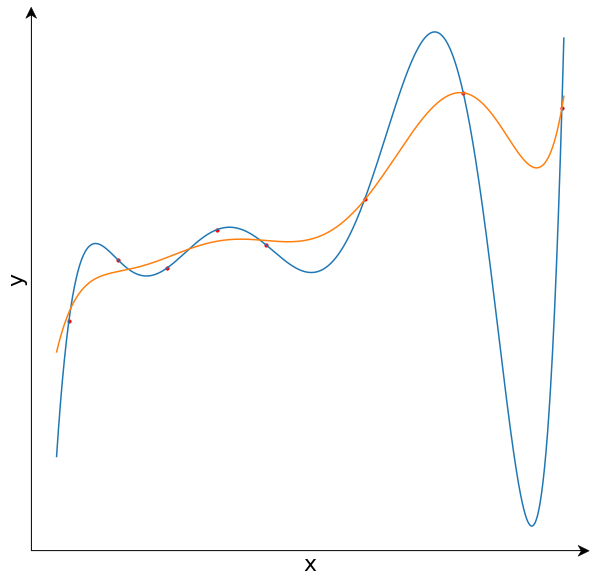
\includegraphics[width=8cm, height = 6cm]{images/regularization.png}
	\centering
	\caption{Regularization illustrated by the polynomial regression example. The blue graph shows 7-degree polynomial with no regularization; the orange one is being yielded by the similar model, but with an added $L_2$ regularizer. The second function is smoother, and intended to generalize better. Note, that it fits the training data worse.}
\end{figure}

Aside from model-specific methods like Dropout, regularization is mostly being implemented as a penalty to model weights:
\[\mathcal{L}^+(W, \mathcal{X}) = \mathcal{L}(W, \mathcal{X}) + \lambda \mathcal{R}(W) \]
where $ \mathcal{L} $ is a loss function and $ \mathcal{R} $ is a regularization term dependant on model weights norm. During training of a regularized model, their sum $\mathcal{L}^+$ is being optimized instead. Parameter $\lambda$ determines the balance between optimizing a loss or a model weight norm. In practice models with a lower weight norm tend to generalize better.

The most widely used regularization terms are $L^1$ and $L^2$ weight norms. $L^1$ directs individual weights towards zero, producing sparse weight vectors, while $L^2$ produces diffuse vectors of small values; sometimes their sum $\lambda_1||W|| + \lambda_2||W||_2^2$, also known as Elastic regularization, is being used.


\subsection{Cross-Validation}

Cross-Validation is a more advanced technique of obtaining a model performance estimation on validation data. Instead of a strict train/validation split, data are being divided into $k$ \textit{folds}---pieces of roughly the same size. During a cross validation process, a model is being $k$ times trained on $k-1$ folds and validated on the last one, different from used in previous iterations.

\begin{figure}[h]
	\centering
	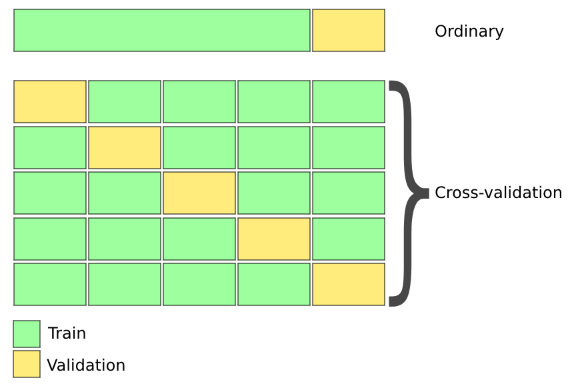
\includegraphics[scale=0.5]{images/cross_validation.png}
	\caption{5-fold cross-validation illustrated.}
\end{figure}

The mean value of $k$ estimations obtained during the cross validation is expected to be more precise and less biased overall model performance estimation. The models obtained during cross validation are also may be combined into an ensemble.

\subsection{Model Ensembling}

Ensembling is a technique commonly used with conventional ML methods, such as decision trees or Bayesian models. The point is to train several models and aggregate them in a certain way---output mean, majority vote, AND or OR rules, etc. While there are wide variety of a model combining, even primitive majority vote method can be beneficial.

Let the $A(x) = \{f_i(x)\}, i \in \hat{\text{N} }$ be the ensemble of N models which perform a binary classification. Let $x_i = \mathbb{I}[f_i \text{ classified wrong}] \sim Bernoulli(p)$ be the random variable. $\mathbb{E}[x_i] = p$, $\sigma^2[x_i] = p(1-p)$. Define $X = \frac{1}{\text{N} } \sum_{i = 1}^{\text{N} } x_i$. Assuming that all $f_i(x)$ misclassifications follow the same distribution $Bernoulli(p)$: $\mathbb{E}[X] = p$, $\sigma^2[X] = \frac{p(1-p)}{\text{N} }$.

By adding more and more models to the ensemble the error distribution will tend to constant. If $p < 0.5$, the error probability will decrease the more models there are in the ensemble. While the two assumptions made there---identical error distributions of all individual models and their independency---are naive, in practice ensembles tend to generalize better.

\begin{figure}[h]
	\centering
	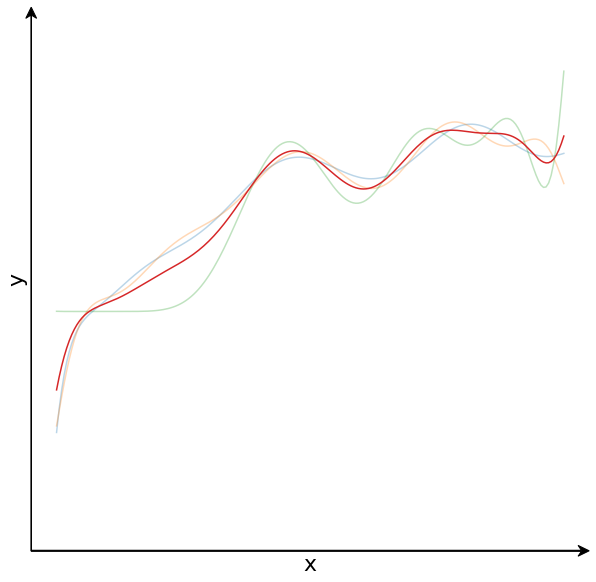
\includegraphics[scale=0.35]{images/ensembling.png}
	\caption{Model averaging illustrated. By averaging several models a smoother function may be obtained.}
\end{figure}

Another explanation why ensembling works is that individual models represent noisy functions. By averaging several complex-relief functions the smoother function is being obtained. Same as in case of regularization, smoother functions tend to generalize better.

Another practical observation is that ensembles tend to work better if their individual models are more diverse. Therefore, individual estimators are being trained on differently sampled data and/or with different hyperparameters, or sometimes they are being represented by completely different architectures.

\chapter{State of the Art}

In the previous chapter basic Machine and Deep learning techniques were introduced. Leaning on those basics, now specific model architectures can be described along with enhanced training techniques. In this chapter the attention will be given to the models employed to solve the task together with the Adam optimizer and Batch Normalization.

\section{Batch Normalization}

\subsection{Motivation}

\textit{Covariate shift} is a situation when a learning system receives an input from a distribution it wasn't trained on\cite{covariate_shift}. This negatively affects a model performance both during training and inference time, since the model starts to re-adapt to a new distribution or to yield biased results respectively. 

Szegedy and Ioffe\cite{batchnorm} extend this definition and apply it to individual neural network parameterized layers. A neural network output may be viewed as an output of several nested subnets:
\[l(u) = F_2(F_1(u, \Theta_1), \Theta_2)\]
where $F_1$ and $F_2$ are two arbitrary transformations and $\Theta_1$ with $\Theta_2$ are their weights. Learning $\Theta_2$ may be seen as training a subnet $F_2(x, \Theta_2)$ on $F_1$ outputs. Assuming $x = F_1(u, \Theta_1)$ a gradient update after a SGD step will be:
\[\Theta_2 \longleftarrow \Theta_2 - \frac{\lambda}{m}  \sum_{i=1}^{m} \frac{\partial F_2(x_i, \Theta_2)}{\partial \Theta_2}\]
which is exactly equivalent to updating a neural network with weights $\Theta_2$ taking $x_i$ as input. Therefore, a constant input distribution is desirable not only for a whole system, but also for all its subparts.

The authors of the paper named this problem an \textit{internal covariate shift}. The cause of this problem is that an output of a layer is heavily dependent on weights of all preceding layers. Any small change applied to weight of a previous layer may significantly affect an input distribution of succeeding layers, and the effect will amplify with a neural network depth. Fluid input distribution slows training down and fluctuates weights, wasting resources on re-adapting to a new input distribution every time it changes.

Another problems they address are vanishing and exploding gradients. While vanishing gradients were briefly described in the previous chapter, \textit{gradient explosion} wasn't mentioned yet. It's a situation when during backpropagation a gradient exponentially grows from layer to layer. This mostly occurs due to too high initial weight values, which lead to high activations and thus high multipliers to the gradient during backprop. Architectures utilizing skip connections are more resilient to this problem\cite{exploding_gradient}; another solutions include proper weight initialization\cite{xavier_init}\cite{he_init}.

\subsection{Problem Addressing}

The method proposed by Szegedy and Ioffe involves addressing the problem directly. Before feeding a data batch to next layer, it is being artificially standardized:
\[x \longleftarrow \frac{x - \hat{x}}{\sqrt{Var(x) + \epsilon}}\]
where $\hat{x}$ is a batch mean, $Var(x)$ is a batch variance and $\epsilon$ is a smoothing added to avoid division by zero. According to LeCun's "Efficient Backprop"\cite{efficient_backprop}, this method is meant to speed up convergence.

Plain data standardization may hurt performance of models which utilize sigmoid activation functions. This transformation restricts data range to a linear segment of such a function. To restore the model representational power, the authors added trainable data scale and shift:
\[x \longleftarrow \gamma\frac{x - \hat{x}}{\sqrt{Var(x) + \epsilon}} + \beta\]
where $\beta$ and $\gamma$ are trainable parameters. Note, that this parameters allow to re-learn original data distributions in case they were optimal.

All operations performed by a \textit{Batch Normalization} (or BatchNorm, BN) are differentiable, and BN may be inserted into a neural network as a further layer. This layer, as well as Dropout\cite{dropout}, works differently during training and test time. During training time, mean and variance estimations are being computed based on a batch statistics. In parallel, the layer updates exponential moving averages of data mean and variance:
\[\mu \longleftarrow m \mu + (1 - m) \hat{x}\]
\[\sigma \longleftarrow m \sigma + (1 - m) \sqrt{Var(x)}\]
where $m$ denotes \textit{momentum}, a value in range between $0$ and $1$, typically 0.99. Moving averages are needed for using in inference time, since it's more common then to feed an ANN with individual samples.

\subsection{Pros and Cons}

\begin{figure}
	\centering
	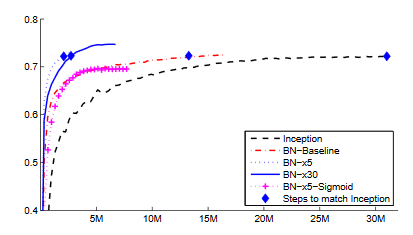
\includegraphics{images/batchnorm_performance.png}
	\caption{Comparison of BN-accelerated models with the baseline taken from the BN paper\cite{batchnorm}. The baseline model was the Inception\cite{going_deeper}; BN-baseline is the Inception with BN before each non-linearity; BN-x5 is the BN-baseline modified to accelerate training (no dropout, reduced $L_2$ regularization, $\times$5 larger initial LR, more aggressive LR decay, etc.); BN-x30 is BN-x5, but with LR increased by factor 30 instead of 5; BN-x5-Sigmoid is the BN-x5 but with ReLUs replaced by sigmoid non-linearity. BatchNormalized models show significant boost both in terms of training speed and accuracy relative to the baseline model.}
\end{figure}

Explicit data normalization brings following benefits:

\begin{itemize}
	\item \textbf{BN addresses vanishing and exploding gradients}. The influence of parameter scale is being significantly reduced, since an information passed through is being normalized to a certain scale. This prevents a model from being stuck into saturated regimes of its sigmoid nonlinearities, and keeps gradient scale in range during backpropagation. This stabilizes training and allows to give less attention to the weight initialization.
	\item \textbf{BN enables higher learning rates}. Higher weight values lead to smaller gradients:
	\[\frac{ \partial \text{BN}((aW)u)}{\partial W} = \frac{\partial \text{BN}((aW)u)}{\partial (aW)}\frac{\partial (aW)}{\partial W}\]
	\[\frac{\partial \text{BN}((aW)u)}{\partial(aW)} = \frac{1}{a}\frac{\partial \text{BN}((aW)u)}{\partial W}\]
	Coupled with the fact that BN prevents gradient explosion, higher weight values will gradually decrease their updates, allowing to multiply them with the higher learning rate.
	
	\item \textbf{BN applies a slight regularization effect}. An individual sample is being influenced by another samples in batch through standardizing by common mean and variance estimations. Thus, during training transformations of this sample are not deterministic.
	
	\item \textbf{BN accelerates training}. Aside from increased learning rates, regularizing effect caused by BN may be sufficient to decrease Dropout rate or to exclude Dropout completely, same as other regularization methods.
	
\end{itemize}
Despite the significant benefits brought by BN, it has its own drawbacks:
\begin{itemize}
	\item \textbf{BN sets a lower bound to the batch size}. To get precise mean and variance estimations, batch sizes have to be higher than a certain threshold. At the same time, large batch sizes are not always possible for RAM-hungry architectures
	\item \textbf{BN works differently during training and inference time}. While Dropout is being just turned off during inference, BN continues to interfere into the data flow inside the model. This may complicate the model interpretation and architecture tuning.
\end{itemize}

Ultimately, it's may be concluded that the benefits outbalance named drawbacks, since BN has begun a very common element of neural network architectures.

\section{Adam Optimizer}

While the gradient descent guarantess non-negative progress if being fed with the whole dataset, it has got some space for further improvements both in terms of convergence speed and stability.

\subsection{Momentum and Nesterov}

SGD method is often being met accompanied by "rolling down the hill" analogy. But this analogy isn't completely accurate---SGD updates weights using the gradient value directly. The more correct analogy would be "sliding down the hill", since once the loss value gets on plateau, gradients become small and training starts to stagnate. It's worth to recall what the vanilla SGD update looks like:
\[W \longleftarrow W - \lambda \nabla W\]

The faster algorithm\cite{learning_representations} may be obtained by utilizing the "rolling" analogy. If several computed gradients point in similar direction, it's likely that following updates also will be in similar direction. Instead of memorizing $n$ last updates, the exponential moving mean of gradients is being used as a compact way to obtain an estimation of update statistics:
\[v \longleftarrow \mu v + (1 - \mu) \lambda \nabla W\]
\[W \longleftarrow W - v\]
$(1 - \mu) \lambda$ term is often being referred simply as $\lambda$. $\mu$ there denotes \textit{momentum}, a term responsible for the speed of accumulated statistics changing or, in terms of the "rolling" analogy, coefficient of friction.

While the Momentum variation of the standard SGD almost always enjoys faster and more stable convergence (due to zig-zag tencencies suppression and a potential to overcome plateaus), there exist further improvements. One of them is the \textbf{Nesterov Accelerated Gradient (NAG)}\cite{nesterov} descent. NAG computes the gradient at the coordinates \textit{after} integration:
\[v \longleftarrow \mu v + \lambda \nabla (W - \mu v)\]
\[W \longleftarrow W - v\]
The idea is that update is to change weights approximately by the term $\mu v$. Hence, computing the gradient at this point will allow to "look ahead" and move faster in case the of loss function relief going down steeper, or move slower in case if it's not.

\subsection{Adaptive Methods}

Another way to improve convergence is to vary the learning rate for different weights according to their update statistics. The most simple example is the Adagrad\cite{adagrad}, which accumulates gradients to use them for per-parameter LR scaling:
\[G \longleftarrow G + (\nabla W)^2\]
\[W \longleftarrow W - \lambda \frac{\nabla W}{\sqrt{G} + \epsilon}\]
where $G$ is the cache of accumulated update statistics and $\epsilon$ is a smoothing. The square root is necessary to prevent a too aggressive growth of $G$ values. To avoid a monotonic cache growth (and thus training slowdown), instead of sum the moving mean of squared gradients is being computed:
\[G \longleftarrow \rho \cdot G + (1 - \rho) \cdot (\nabla W)^2\]
where $\rho$ is a hyperparameter. The algorithm with this modification is being known as RMSProp\cite{rmsprop}.

Per-parameter update scaling allows to be more robust against \textit{saddle points}---the points in space where the first derivatives by all parameters are (almost) zero, but the second derivatives are not and vary in sign. While not being (local) minima, they may lead to stagnation of training provided by momentum-based algorithms.

\subsection{Adam}

Adam\cite{adam} (from "adaptive moment estimation") emerged as an algorithm trying to combine advantages of both momentum and adaptive algorithms. It utilizes estimations of first (like the Momentum SGD algorithms) and second (like the Adagrad algorithm family) gradient moment estimations. A simplified Adam update may be written this way:
\[m \longleftarrow \beta_1 m + (1 - \beta_1) \nabla W\]
\[v \longleftarrow \beta_2 v + (1 - \beta_2) (\nabla W)^2\]
\[W \longleftarrow W - \lambda \frac{m}{\sqrt{v} + \epsilon}\]
where $\beta_1$, $\beta_2$ and $\epsilon$ are hyperparameters (the paper recommends 0.9, 0.999 and \num{1e-8} respectively).

One of the Adam novelties is the \textit{bias correction} mechanism introduced to obtain unbiased first and second gradient moments estimations. Being initialized with zeros, they suffer from biasing towards zero until they "warm up" after a certain number of updates. To avoid this, additional step is being required for an each moment update before using it for a weight update.

The full weight update may be written as:
\[m^{(t)} \longleftarrow \beta_1 m^{(t-1)} + (1 - \beta_1) \nabla W^{(t-1)}\]
\[v^{(t)} \longleftarrow \beta_2 v^{(t-1)} + (1 - \beta_2) (\nabla W^{(t-1)})^2\]
\[m^{(t)}_c \longleftarrow \frac{m^{(t)}}{1 - \beta_1^{t}}\]
\[v^{(t)}_c \longleftarrow \frac{v^{(t)}}{1 - \beta_2^{t}}\]
\[W^{(t)} \longleftarrow W^{(t-1)} - \lambda \frac{m^{(t)}_c}{\sqrt{v^{(t)}_c} + \epsilon}\]
where $m^{(t)}_c$ and $v^{(t)}_c$ represent unbiased first and second moments estimations at the $t$\textsuperscript{th} iteration.

\subsection{Adam Features}

\begin{itemize}
	
	\item \textbf{Adam combines both adaptivity of Adagrad family and update speed of Momentum algorithms}. Thanks to accumulated first gradient moment statistics, Adam is able to get through plateaus and shallow local minima, while the per-parameter update scaling coupled with stochastic jitter allow to quickly escape saddle points.
	\item \textbf{Update step is bounded and independent on gradient scale.} The update step is basically $- \lambda \cdot E[ \nabla W] / \sqrt{ E[(\nabla W)^2] }$. Since for the random variable $X$ there is a relation $| E[X] / \sqrt{ E[X^2]} | \leq 1 $, the update step is approximately limited by $\lambda$:
	\[\Delta W \approx - \lambda \cdot \frac{E[ \nabla W]}{\sqrt{ E[(\nabla W)^2] }} \implies |\Delta W| \lessapprox \lambda \]
	\item \textbf{Adam doesn't require careful hyperparameter tuning}. The proposed values for $\beta_1, \beta_2 \text{ and } \epsilon$ work well in most of tasks and could be left untouched. At the same time, thanks to the update scale bounding it's easier to pick the right learning rate.
\end{itemize}

\section{Deep Residual Networks}

\begin{figure}[h]
	\centering
	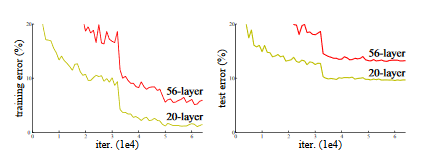
\includegraphics{images/degradation.png}
	\caption{Degradation problem illustrated, plots taken from the paper\cite{resnet}. The plots clarify that the problem isn't related to overfitting, since deeper models are harder to optimize for training data.}
\end{figure}

After the AlexNet\cite{alexnet} won the ImageNet in 2012, researches studied the possibilities of further expanding of CNN capabilities. It appeared, that a model depth is very important\cite{vgg}\cite{going_deeper} for its expressive power, along with vertical scaling being easy to implement to design models for different purposes.

But the sequential layer arrangement limits training capabilities of CNNs---it appears, that sequential CNNs have an upper bound of layer count, beyond which their performance starts to decrease. CNNs, which suffer from this kind of degradation, cannot achieve not only same validation results as shallower ones---their \textit{training} results are also worse.

The degradation problem may be explained as a situation when during training first $n$ model layers extract as much useful features as it is possible, and the optimal transformation the rest of layers can learn is an identity. But learning such a simple transformation by a sequence of nonlinear layers appears not to be possible.

He et al. in their breakthrough work\cite{resnet} addressed this problem by introducing a \textit{residual block}. Instead of non-linear transformation $y = \mathcal{F}(\{W_i\}, x)$ a layer block can learn a residual transformation:
\[y = \mathcal{F}(\{W_i\}, x) + x\]
where $y$ is a block output, $x$ is a block input and $\mathcal{F}(\{W_i\}, x)$ represents a transformation of input by a sequence of ConvLayers. The $+$ operation is mostly being implemented by an element-wise sum of two tensors---this is computationally efficient, introduces no additional parameters and is enough to address the problem; albeit another implementations may exist, like concatenation followed by $1 \times 1$ convolutions.

\begin{figure}[h]
	\centering
	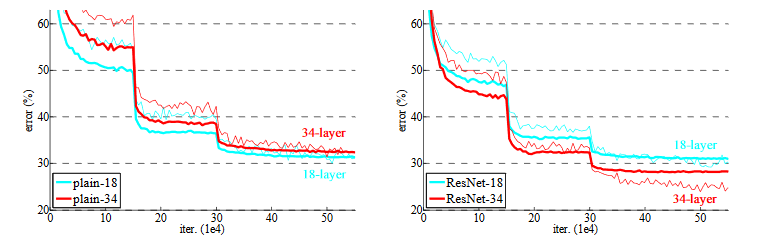
\includegraphics[width=\textwidth]{images/residual_results.png}
	\caption{Comparison of two CNN pairs---plain 18-layer, plain 34-layer and their residual variants. Plot is taken from the paper\cite{resnet}. Skip connections bypass every two layers. While providing no additional parameters, residual networks show better results.}
\end{figure}

Skip connections allow to learn a non-linear transformation if it yields a better result, or to learn zero weights if identity mapping is the best mapping that could be learned---and thus to not degrade an ANN performance in the worst case. This concept allows to train CNNs of an arbitrary depth---the ImageNet 2015 winner was an ensemble of 152-layer ResNets, while He et al. in their work explored models with more than 1000 layers.

\section{Densely Connected Convolutional Networks}

\begin{figure}[h]
	\centering
	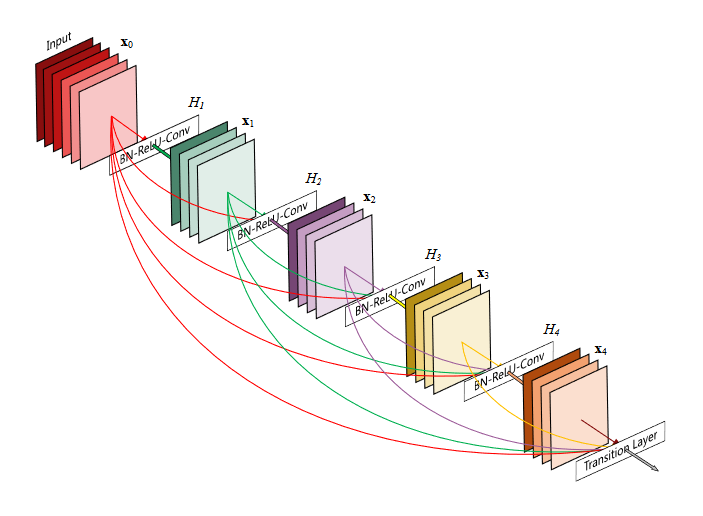
\includegraphics[scale=0.66]{images/dense_block.png}
	\caption{A 5-layer dense block with growth rate = 4. Picture from the DenseNet paper\cite{densenet}.}
\end{figure}

\subsection{Motivation}

DenseNet\cite{densenet} is a further successor of ResNet, expanding its original concept to setting a skip connection between each pair of layers of matching size. The dense connectivity enhances an information flow and decreases a number of parameters, which allows to train the network with more ease and achieve better results than sequential or residual networks. 

The network emerged as a distillation of several methods\cite{resnet}\cite{stochastic_depth}\cite{highway_net}, employed to allow to build more deep neural networks. While being different, most of them shared a thought of introducing skip connections between certain pairs of layers. The authors of DenseNet went further, and installed a skip connection between \textit{all} pairs of layers which were possible.

The counter-intuitive benefit is that the new model contains \textit{less} parameters than comparable sequential and residual ones. The authors' explanation is that a CNN layer passes to next layer both newly generated feature maps and maps preserved from previous layers. This significantly increases parameter count, dedicating some of parameters to learning re-encoding an information to be preserved. DenseNet introduces an explicit distinguish between newly generated and preserved feature maps---its convolutions, while taking all previously generated feature maps as input, produce relatively shallow output (typically 4-32 feature maps), which is then being added to the common stack. The final layer makes its decision leaning on all feature maps generated by the model.

Another big advantage of the proposed architecture is that during backpropagation gradient flows directly from the last layer to an each layer in the network, speeding up the training significantly and, according to the paper, applying a slight regularizing effect.

\subsection{Key Architecture Elements}

Each CNN consists of several non-linear transformations, each of which is mostly being a combination of a convolutional layer, batch normalization and a ReLU activation function. Such a combination authors of the model refer as $\mathcal{H}_l(\cdot)$, where $l$ is a layer index. With denoting a $l$\textsuperscript{th} layer output as $x_l$, a sequential CNN transformation may be written as $x_l = \mathcal{H}_l(x_{l-1})$.

As it was mentioned, Residual Networks compute a sum of a non-linear transformation and a residual block input:
\[x_l = \mathcal{H}_l(x_{l-1}) + x_{l-1}\]
But the authors of the paper\cite{densenet} argue that a skip connection implemented as a sum may impede the information flow. Instead, they propose to apply a non-linear transformation to concatenated outputs of all previous transformations:
\[x_l = \mathcal{H}_l([x_0, x_1,\dots,x_{l-1}])\]
where $[x_0, x_1,\dots,x_{l-1}]$ denotes feature maps produced by previous transformations, concatenated along the depth axis.

The non-linear transformation there is being implemented as Batch Normalization + ReLU + $3 \times 3$ Conv layers---the layer block utilizes the pre-activation scheme, which is intended to improve generalization\cite{identity_mappings}. The $\mathcal{H}(\cdot)$ output depth is kept constant, and is being referred as a network's \textit{growth rate}, or $k$---a hyperparameter responsible for a model "width".

The authors also found it useful to insert a "bottleneck" transformation before mentioned $3 \times 3$ convolutional block to decrease both a parameter count and computational complexity. This transformation also utilizes BN + ReLU + Conv scheme, albeit with $1 \times 1$ convolution producing $4k$ feature maps. The BN-ReLU-($1 \times 1$ Conv)-BN-ReLU-($3 \times 3$ Conv) composed transformation further will be referred as a \textit{convolutional block}.

The DenseNet is divided into several \textit{dense blocks}. A dense block is a sequence of convolutional blocks which accept and produce feature maps of a specific size. Since spatial sizes of the feature maps are identical, they can be freely concatenated. Each convolutional block in a dense block accepts an input, produces its output and concatenates it with its input. The new stack obtained will be sent to the next convolutional block as input.

The information compression between dense blocks is being implemented by \textit{transition blocks}. Transition block is composed of BN-ReLU-($1 \times 1$ Conv)-(2 $\times$ 2 Avg Pooling) layers. While average pooling shrinks data spatially, the $1 \times 1$ convolutional layer compresses data along the depth axis, producing less layers than it accepts. Being a trainable dimensionality reductor, it additionally enhances the network compactness.

\subsection{Pros and Cons}

The novel architecture brings following benefits:

\begin{itemize}
	\item \textbf{Accuracy}. DenseNet appeared to be a very powerful architecture, beating\cite{densenet} state-of-art architectures at the moment of the paper publication.
	\item \textbf{Training Ease}. DenseNet trains itself faster and more reliably thanks to the low parameter count and more efficient layer arrangement.
	\item \textbf{Simplicity}. DenseNet doesn't contain gates as Highway Nets or recursive patterns as FractalNets. Its architecture pattern is only slightly more complex than ResNet's is.
\end{itemize}

While exceeding state-of-art models in most of benchmarks, DenseNet suffers significant \textbf{RAM consumption}. DenseNets are relatively deep in comparison with competitive models, and that leads to the higher RAM consumption during training, since it's needed to keep more feature maps in memory during backpropagation. This limits maximum batch size and thus may limit BN performance, while the model is relying heavily on them.

\subsection{Specialized Dropouts}

While state-of-art models mostly rely on Batch Normalization, skip connections and extensive data amounts to avoid overfitting, some tasks may require training on smaller data sets and thus explicit regularization. There is a work\cite{specialized_dropouts}, which describes a DenseNet-specific technique of the Spatial Dropout layer arrangement leading to higher generalization using the prior knowledge of how the model works.

The first intuition behind the work stands on analysis of how DenseNet convolutions are arranged. In particular, channel counts with which convolutions operate grow gradually from start to end of a dense block. Skipping feature maps at a dense block beginning may hurt the model's performance, so it makes sense to skip them with increasing probability along the dense block. That led to the scheme which places the Spatial Dropouts before each convolution block with an increasing dropout rate the further the ConvBlock is from its input transition layer. The authors of the paper refer this scheme as $v_1$.

Another intuition originates in observations made by the DenseNet authors, reflected in their paper\cite{densenet}. Later dense blocks tend to assign lower weights to transition block outputs, while feature maps generated "locally" tend to gain higher attention. Furthermore, the weights assigned by the final layer to inputs tend to be higher for newer feature maps. That led to another dropout scheme, which skips feature maps before each convolution block depending on the distance between this feature map source and the ConvBlock---the "elder" the feature map is, the higher will be chance of it being skipped. This preserves newly generated feature maps from skipping along with getting rid of old and supposedly redundant information. This scheme is being referred as $v_3$ in the paper.

According to the paper, $v_2$, which was the inverse of $v_1$, with decreasing dropout rates meant to keep the number of dropped feature maps constant, didn't improve the model. But models with $v_1$ and $v_3$ both exceeded original results, with $v_3$ being the best. Furthermore, the authors extend their approach to other models, such as AlexNet, VGG16 and ResNet variants, and show that $v_2$ analog which is intended to reduce the total randomness brought by dropout layers helps to improve generalization of the models.

\section{Mask R-CNN}

\subsection{Purpose}

While the previously described models were designed for image classification or regression, the computer vision tasks do not end there. Most of them can be split into four sorts:
\begin{itemize}
	\item \textbf{Classification.} Given a certain input, yield a single value or a vector according to the image semantics. Regression and multi-class label assignment arguably can be also attributed there (ResNet, DenseNet,\dots).
	\item \textbf{Semantic Segmentation}. Classify an every pixel on image. Image regions, belonging to the same class but different class instances, are not discriminated (SegNet, U-Net,\dots).
	\item \textbf{Object Detection}. Detect all objects on image, classify and find their bounding boxes (Regions with CNN, Fast R-CNN, Faster R-CNN).
	\item \textbf{Instance Segmentation}. Detect all objects on image, classify and find their masks (Mask R-CNN).
\end{itemize}

\begin{figure}[ht]
	\centering
	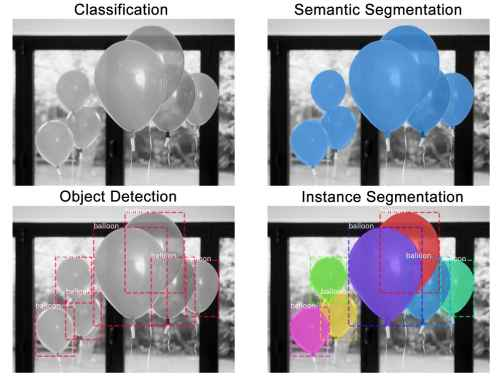
\includegraphics[scale=0.75]{images/segmentation.jpeg}
	\caption{The four CV tasks illustrated. Picture from\cite{splash_of_color}.}
\end{figure}

The Mask R-CNN architecture is dedicated to solve exactly the last task. Since Instance Segmentation presents a combination of previous tasks, such as Object Detection and Semantic Segmentation, Mask R-CNN borrows a lot from architectures designed for them. Before moving on Mask R-CNN architecture details, it's worth to say a word about its predecessors, since this architecture is a result of a gradual evolutionary development.

\subsection{Predecessors}

\subsubsection{Regions with CNN}

One of the first successful attempts of applying CNNs for object detection is a Regions with CNN\cite{rcnn} architecture, or R-CNN. The algorithm was based on a conventional region proposal method which extracted 2000 regions from an input image. Every extracted region then was padded, resized and fed to a pre-trained deep CNN. The CNN produced a 4096-dimensional feature vector, used both for classification and bounding box regression.

\begin{figure}[h]
	\centering
	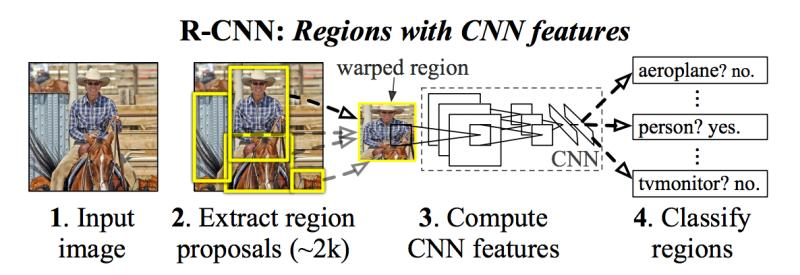
\includegraphics[scale=0.5]{images/rcnn.jpeg}
	\caption{The Regions with CNN scheme. The algorithm extracts region proposals from an original image, feeds them to CNN and classifies them by multiple SVMs. Picture from\cite{rcnn}.}
\end{figure}

The final class prediction was produced by binary-classifying SVMs for each class. To predict a bounding box, the authors employed ridge regression to predict four values: $x$, $y$, $w$, $h$. Those values are offsets of bounding box center and sizes relative to the proposed region boundaries.

While being relatively effective in comparison with its competitors, the architecture's major drawback was its performance. It took roughly \textit{one minute} to process a single image due to the huge number of CNN applications, which limited its usability.

\subsubsection{Fast R-CNN}

\begin{figure}[h]
	\centering
	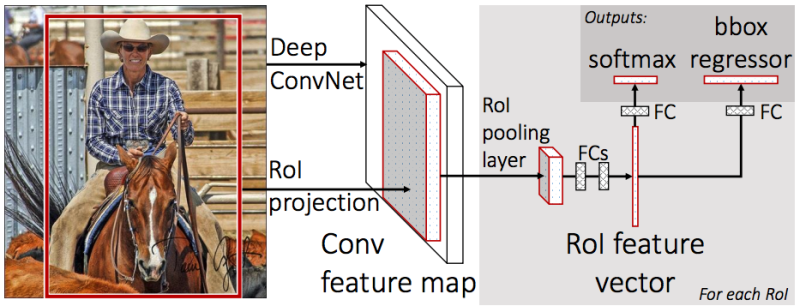
\includegraphics[scale=0.5]{images/fast_rcnn.png}
	\caption{The Fast R-CNN architecture scheme. Instead of repeating CNN applications, the model applies the CNN only once. The proposed regions are being projected to the CNN output, pooled, fed to fully-connected layers and finally passed to the two heads for classification and bounding box regression. Picture from\cite{fast_rcnn}.}
\end{figure}

The computational overhead of R-CNN was caused primarily by numerous CNN applications on overlapping region proposals. To optimize computations, the Fast R-CNN\cite{fast_rcnn} applies a fully-convolutional CNN on a whole image at once.

This is possible due to the fact, that a certain region on an input image corresponds to a certain region on a fully-convolutional CNN output. This allows to map proposed regions to the CNN output instead of applying a CNN on each region proposal distinctly.

Fast R-CNN performs such a mapping followed by the so-called \textbf{RoI Pooling} operation. This operation performs a spatial split of a projected region proposal (of size $h \times w$) to $H \times W$ grid (with a cell of size  $h/H \times w/W$). Each feature map is then being max-pooled with respect to this grid and flattened, resulting in a vector of a fixed size. To obtain a final RoI feature vector, the pooled and flattened values are then being fed to several fully-connected layers.

The rest of the model branches to the two heads: one head for classification and one for regression, and the network is being trained by optimizing a sum of two losses. In result, the Fast R-CNN architecture is being trained end-to-end, instead of multi-stage original R-CNN preparation which was slow, disk space-hungry and didn't include model co-adaptation. What is more significant is that Fast R-CNN showed itself roughly 200 times faster at test time, with the main bottleneck becoming a region proposal algorithm.

\subsubsection{Faster R-CNN}

While being faster than R-CNN, Fast R-CNN still utilized a conventional region proposal algorithm, which limited its performance and didn't make use of features extracted by a CNN. The authors of a new architecture, Faster R-CNN\cite{faster_rcnn}, proposed to generate RoIs by a neural network applied on CNN outputs instead of raw images.

\begin{figure}[h]
	\centering
	
	\begin{subfigure}[b]{.48\textwidth}
		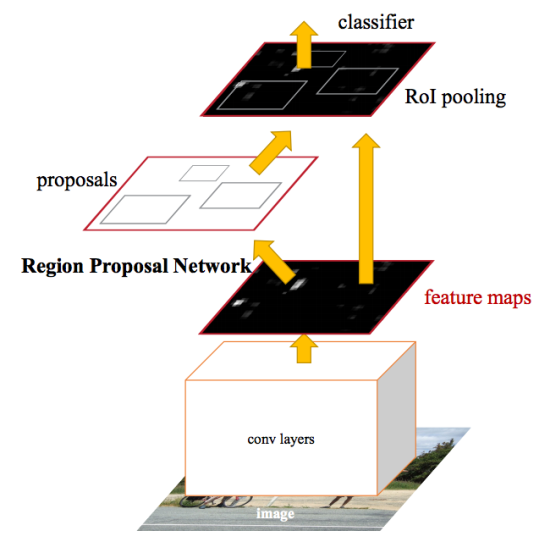
\includegraphics[scale=0.4]{images/faster_rcnn_overall.png}
	\end{subfigure}
	\begin{subfigure}[b]{0.48\textwidth}
		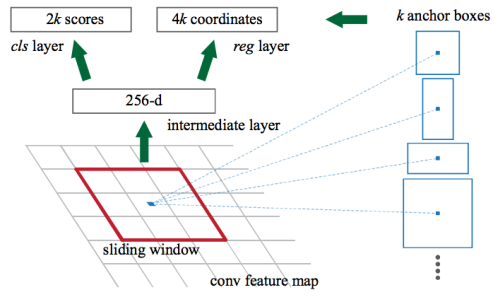
\includegraphics[scale=0.5]{images/anchors.png}
	\end{subfigure}
	
	\caption{Left: The Faster R-CNN architecture brief scheme. The RPN slides over the backbone output and utilises the extracted features to propose regions. The proposed regions are then being processed similarly to Fast R-CNN. Right: The RPN application example. On a certain position for each of $k$ anchor shapes it predicts $2k$ values for "objectness" score (is there any object or not), and $4k$ values for bounding box regression relative to the anchor boundaries. Pictures from \cite{faster_rcnn}.}
\end{figure}

\textbf{RPN}, or a Region Proposal Network, is the main novelty introduced in the Faster R-CNN paper. RPN is a fully-convolutional network which is being slided over feature maps extracted by a "larger" CNN, or a \textbf{backbone}. It consists of a $3 \times 3$ convolutional layer and two distinct output fully-connected layers---box-regression layer (reg) and box-classification layer (cls). Outputs of these layers are based on so-called \textit{anchors}. An anchor is a box region of a certain scale and aspect ratio, which is centered at the current sliding window position.

For an every sliding window position, RPN predicts $4k$ values by its regression layer and $2k$ values by its classification layer, where $k$ denotes an anchor count. For an each anchor, \textit{reg} produces 4 offsets of anchor box coordinates, while \textit{cls} produces 2 values indicating is there any object inside or not. The authors of Faster R-CNN used 3 scales ($128^2$, $256^2$ and $512^2$ $\text{px}^2$ areas with respect to an input image) and 3 aspect ratios (1:1, 2:1, 1:2) in the paper, resulting in $k = 9$. Weights of both RPN heads are shared across an image, and those layers are being implemented as $1 \times 1$ convolutions with $4k$ and $2k$ kernels respectively. Note, that RPN output is invariant to translation and depends only on anchor context. It's also worth to point to the amount of context captured by RPN---a one pixel of VGG16 (used in the paper) output corresponds with $16 \times 16$ area on original image.

After the RPN application there are $WHk$ possible proposals, where $W$ and $H$ are the CNN output width and height respectively. Most of them are overlapping and redundant, and the \textbf{Non-Maximum Suppression (NMS)} procedure is being employed to get rid of noise. NMS takes a proposal list sorted by cls-score and iterates over it, looking for overlapping groups. For each overlapping group NMS selects the single proposal with maximum cls-score and discards the rest which have intersection-over-union with it more than a certain threshold:

\[\text{IoU} = \frac{A \cap B}{A \cup B} > T\]
where $A$ is a max-cls region, $B$ is an another overlapping region and $T$ is a threshold. The rest of proposals is being sorted again and top-N values (typically 2000) are being kept.

The rest of the model is being implemented similarly to Fast R-CNN---obtained proposals are RoI-pooled, passed through fully-connected layers and fed to the two final branches, predicting class and bounding box offset.

Ultimately, to train Faster R-CNN one has to train two CNNs: RPN and Fast R-CNN. The authors of Faster R-CNN proposed several training algorithms, but in the paper they used the following one:
\begin{enumerate}
	\item Initialize the backbone with ImageNet weights and fine-tune backbone + RPN composed network.
	\item Initialize Fast R-CNN (backbone + heads) with ImageNet weights and train it using the RPN obtained from the previous step. Note that after this step RPN and Fast R-CNN are not sharing backbone weights.
	\item Fine-tune RPN with the frozen backbone. Now both networks share the weights.
	\item Freeze the backbone and fine-tune the Fast R-CNN heads.
\end{enumerate}
These four steps are sufficient for most of tasks, and the authors observed no significant improvements after more training iterations.

Despite the sophisticated structure, Faster R-CNN presents both effective and elegant solution in shape of the completely end-to-end trainable network. While being computationally efficient (the authors report 10ms overhead during test time), RPN also represents trainable algorithm utilizing the power of a deep CNN.

\subsection{Architecture Details}

\begin{figure}[h]
	\centering
	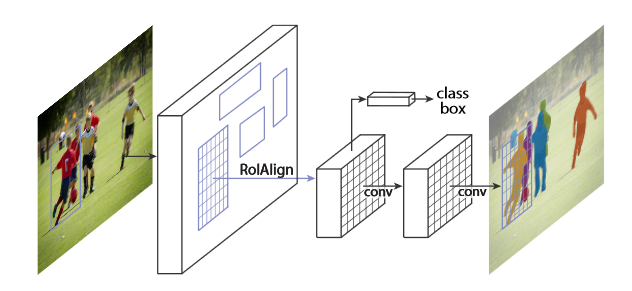
\includegraphics[scale=0.66]{images/mrcnn.png}
	\caption{The Mask R-CNN architecture. Note the additional convolutional layer sequence predicting the masks and the RoI Align layer. Picture from\cite{mask_rcnn}.}
\end{figure}

The Mask R-CNN\cite{mask_rcnn} extends Faster R-CNN by an additional head---the mask predictor. A mask is nothing more than a binary map of N + 1 depth, where N is a number of classes, with an additional class for background. "True" or "False" on a certain position means that this pixel belongs to a certain class. Hence, the mask predictor head is a fully-convolutional CNN with the last layer being a $1 \times 1$ convolution. It's worth to note, that the head predicts masks independently on classification results---i.e. masks do not compete with each other.

Another important change is a new operation employed to replace the RoI Pooling. The original RoI Pool, while performing well for classifying and bounding box prediction, provides a crude quantization of an input data. To keep more spatial information, RoI Pool was replaced by the \textbf{RoI Align} layer interpolating data instead of quantizing.

\subsubsection{RoI Align}

\begin{figure}[h]
	\centering
	
	\begin{subfigure}[b]{.48\textwidth}
		\centering
		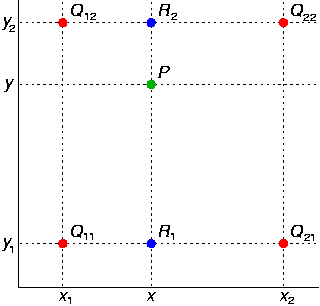
\includegraphics[scale=0.4]{images/bilinear_interpolation.png}
	\end{subfigure}
	\begin{subfigure}[b]{0.48\textwidth}
		\centering
		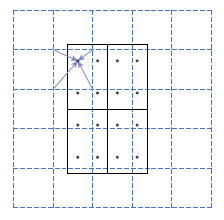
\includegraphics[scale=0.7]{images/roi_align.png}
	\end{subfigure}
	
	\caption{Left: Bilinear interpolation illustration. To interpolate the point, the four neighbours are needed. The interpolation is being computed along the one axis firstly (producing points $R_1$ and $R_2$), and then along another (using $R_1$ and $R_2$), resulting in three linear interpolations. Right: RoI Align example. The solid line represents the proposed region being pooled, while the stroke line delimits the backbone output. Each pooling bin has got four sampling points, each of which gets a bilinearly interpolated values of the feature map pixels. The pooling is being applied on sampling points, not on feature map pixels. Pictures from \cite{bilinear_interpolation} and \cite{mask_rcnn} respectively.}
\end{figure}

The original RoI Pool performs data quantization twice:
\begin{enumerate}
	\item The proposed RoI of arbitrary size is being aligned to fit into feature map region of an integer size
	\item The aligned RoI is then being pooled into fixed number of bins
\end{enumerate}
To save more spatial information, RoI Pool was replaced by RoI Align layer which doesn't perform such quantizations at all. The RoI Align algorithm can be described this way:
\begin{enumerate}
	\item The proposed RoI is being placed over the feature map without align (with corner coordinates being floating point numbers relative to the backbone output)
	\item The region is being divided into fixed number of bins, same as RoI Pooling does
	\item Fixed number of \textit{sampling points} is being selected for each bin. The authors used four sampling points located on intersection of bin thirds
	\item The values for each sampling point are being computed using bilinear interpolation of feature map pixels
	\item Computed sampling point values are being pooled (e.g. with max or average function)
\end{enumerate}
Precise aligning and interpolation instead of quantizing allows to properly align the predicted mask with the object on input image. The authors didn't observe result sensitivity to sampling points number or exact location until no quantization is performed, while the replacing RoI Pool by RoI Align itself showed drastic performance increase.

\subsubsection{Mask Predictor Head}

\begin{figure}[h]
	\centering
	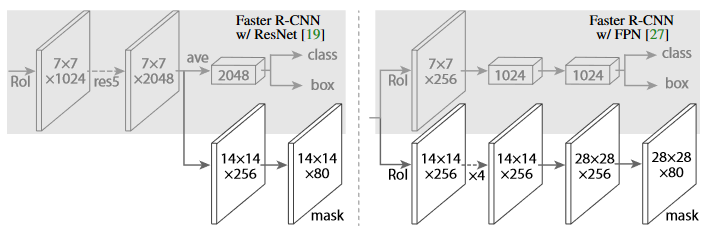
\includegraphics[scale=0.6]{images/mask_predictors.png}
	\caption{The proposed mask predictors for ResNet and Feature Pyramid Network\cite{feature_pyramid_nets} backbones respectively. Arrows denote either convolution, deconvolution or fully-connected layers as can be inferred from context. All convolutions are $3 \times 3$, except the output convolution which is $1 \times 1$. Deconvolutions are $2 \times 2$ with stride 2, all layers use ReLU non-linearity. Picture from\cite{mask_rcnn}.}
\end{figure}

As it was mentioned, the mask predictor is a fully-convolutional CNN, which is implemented similarly as FCNs for semantic segmentation. Nonetheless, the authors found it more profitable to decouple classification and mask prediction processes, unlike how it is in most of semantic segmentation models.

During training, the loss function applied to the last layer is a mean per-pixel binary cross-entropy of the correct class mask only. During inference, the head predicts N masks for each class, while only $n$\textsuperscript{th} mask is being yielded as output, where $n$ is the class predicted by the classifier head. Once the mask is predicted, thanks to RoI Align it can be precisely re-projected to an output image.

\chapter{Practial Part}

This chapter describes an approach used to solve the related task step-by-step. The problem will be decomposed to the several subtasks, and for each of them---from the data preprocessing to the joint scoring itself---the solution will be designed using the methodology described in the previous two chapters.

\section{Task Recapitulation}

The goal of the RA2 Challenge\cite{synapse_ra2} is to design a system able to perform a joint damage assessment by the Sharp/van der Heijde (SvH) method. The assessment system stands on examining selected hands, wrists and feet joints, which are the typical RA targets. The system considers a \textbf{joint erosion} (physical damage of the joint bones) and a \textbf{joint space narrowing (JSE)} (reduction of the free space between joint bones). Each erosion and narrowing region is being scored in range from 0 to 5 and from 0 to 4 respectively. The whole scoring requires 86 examinations yielding the total score in range from 0 to 448.

Note that feet erosion scores are considered per \textit{side} of joint, not the joint itself; the actual feet joint erosion score range is from 0 to 10.

\begin{figure}[h]
	%\centering
	
	\begin{subfigure}[b]{.48\textwidth}
		\centering
		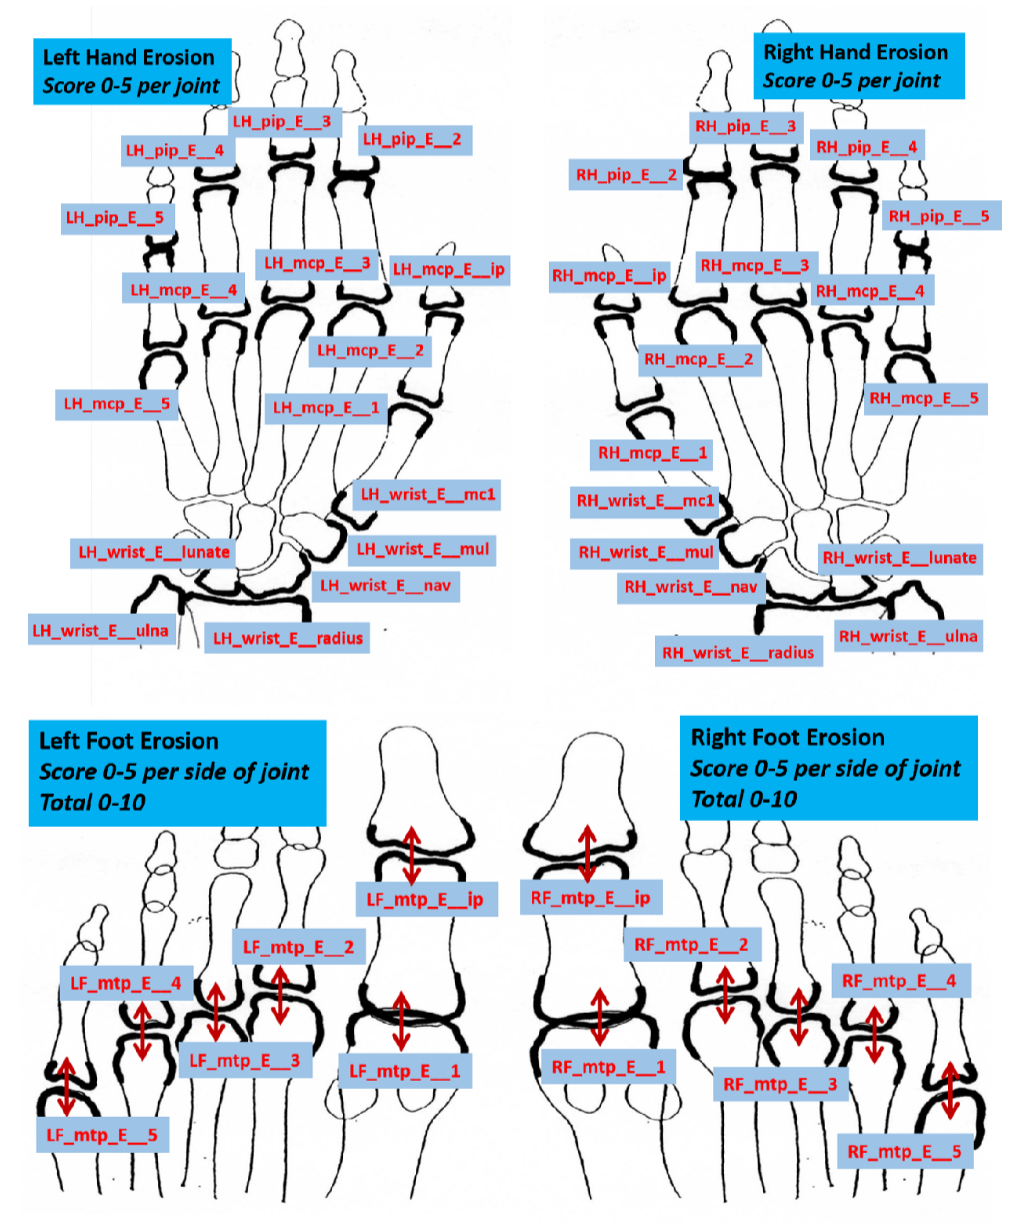
\includegraphics[height = 8cm]{images/erosion_regions.png}
	\end{subfigure}
	\begin{subfigure}[b]{.48\textwidth}
		\centering
		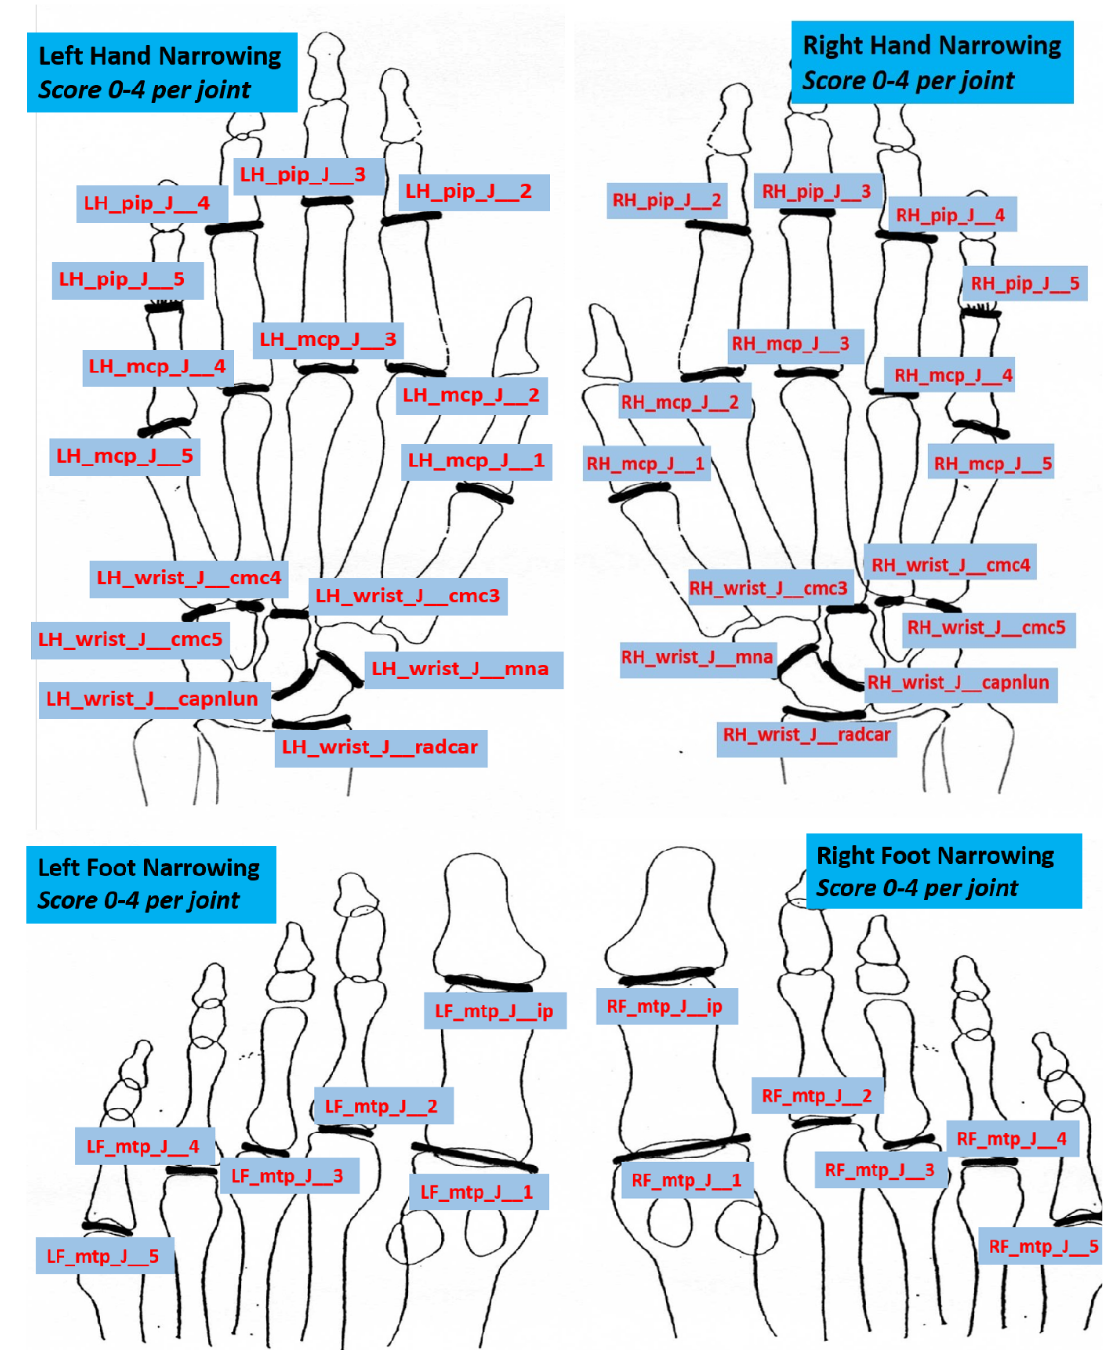
\includegraphics[height = 8cm]{images/narrowing_regions.png}
	\end{subfigure}
	
	\caption{Regions for which erosion or narrowing needs to be assessed. Left: erosion regions. Right: narrowing regions.}
\end{figure}

The challenge consists of 3 subchallenges:
\begin{itemize}
	\item \textbf{Subchallenge 1:} Predict an overall RA damage. Solution assessment metric: weighted MAE
	\item \textbf{Subchallenge 2:} Predict joint space narrowing jointwise. Solution assessment metric: weighted RMSE
	\item \textbf{Subchallenge 3:} Predict joint erosion jointwise. Solution assessment metric: weighted RMSE
\end{itemize}

It's worth to mention that metrics' weights were not publicly available during the challenge.

The solution must be dockerized, pushed to the challenge repository and submitted through the form; submissions are limited to the three per round which is typically a week long. The container should be able to (optionally) train itself and produce the output table; the "Fast lane" unlimited submissions are provided to run the container on a small subset of data and ensure it yields a valid result.

\section{Dataset Overview}

The data set consists of CLEAR and TETRAD studies and contains left hand, right hand, left foot and right foot images of 368 patients, giving 1472 images in total. The only labels available are 86 SvH scores and their erosion/narrowing/total sums per patient. Images vary in size, contrast and sharpness; all of them are oriented similarly per limb. Among the foreign objects there are wrist bone plates, jewelry and labels on images.

\begin{figure}[h]
	\centering
	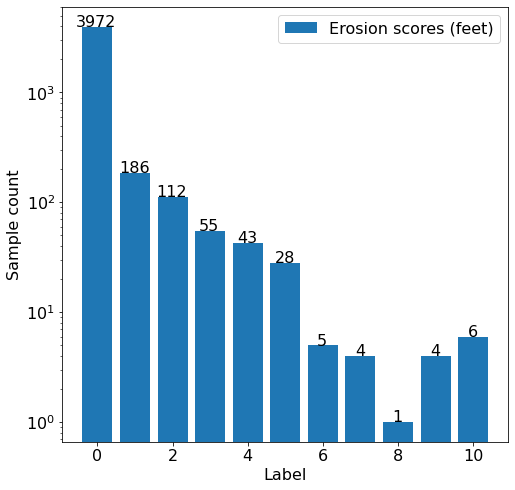
\includegraphics[height=6cm]{images/sample_counts_fe.png}
	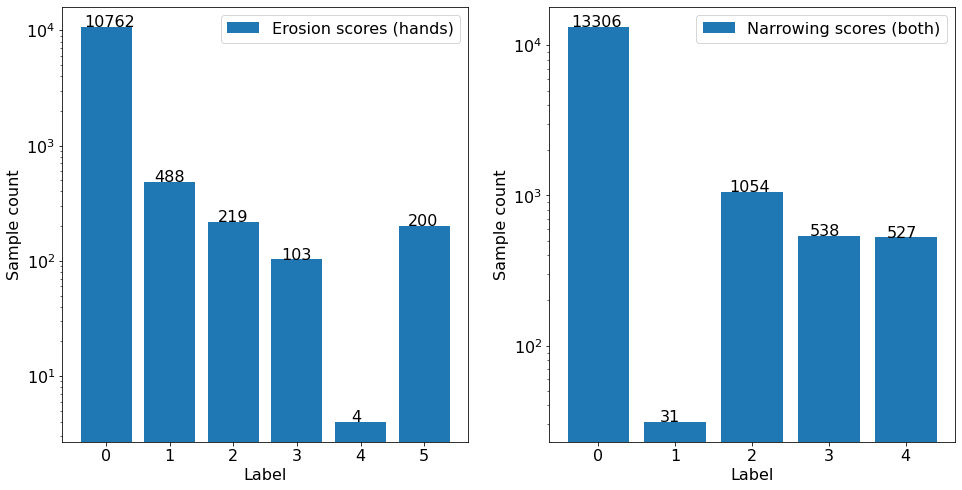
\includegraphics[height=6cm]{images/sample_counts_rest.png}
	\caption{Label values distribution in log scale. Note that for some labels only 1-31 labels are available.}
\end{figure}

The label analysis revealed that \textbf{only 14\% of narrowing and 9\% of erosion scores are non-zero}. That significantly reduces the information amount that could be extracted from the data, and dealing with a prevalence of negative examples is a part of the challenge. There are also labels being assigned only to few images (erosion scores 4 for hands, for example).

It's important to note, that most of erosion and narrowing regions overlap. The only significant difference is the carpal regions, which in case of region extraction from image will have to be processed separately.

\begin{figure}[h]
	\centering
	
	\begin{subfigure}[b]{.48\textwidth}
		\centering
		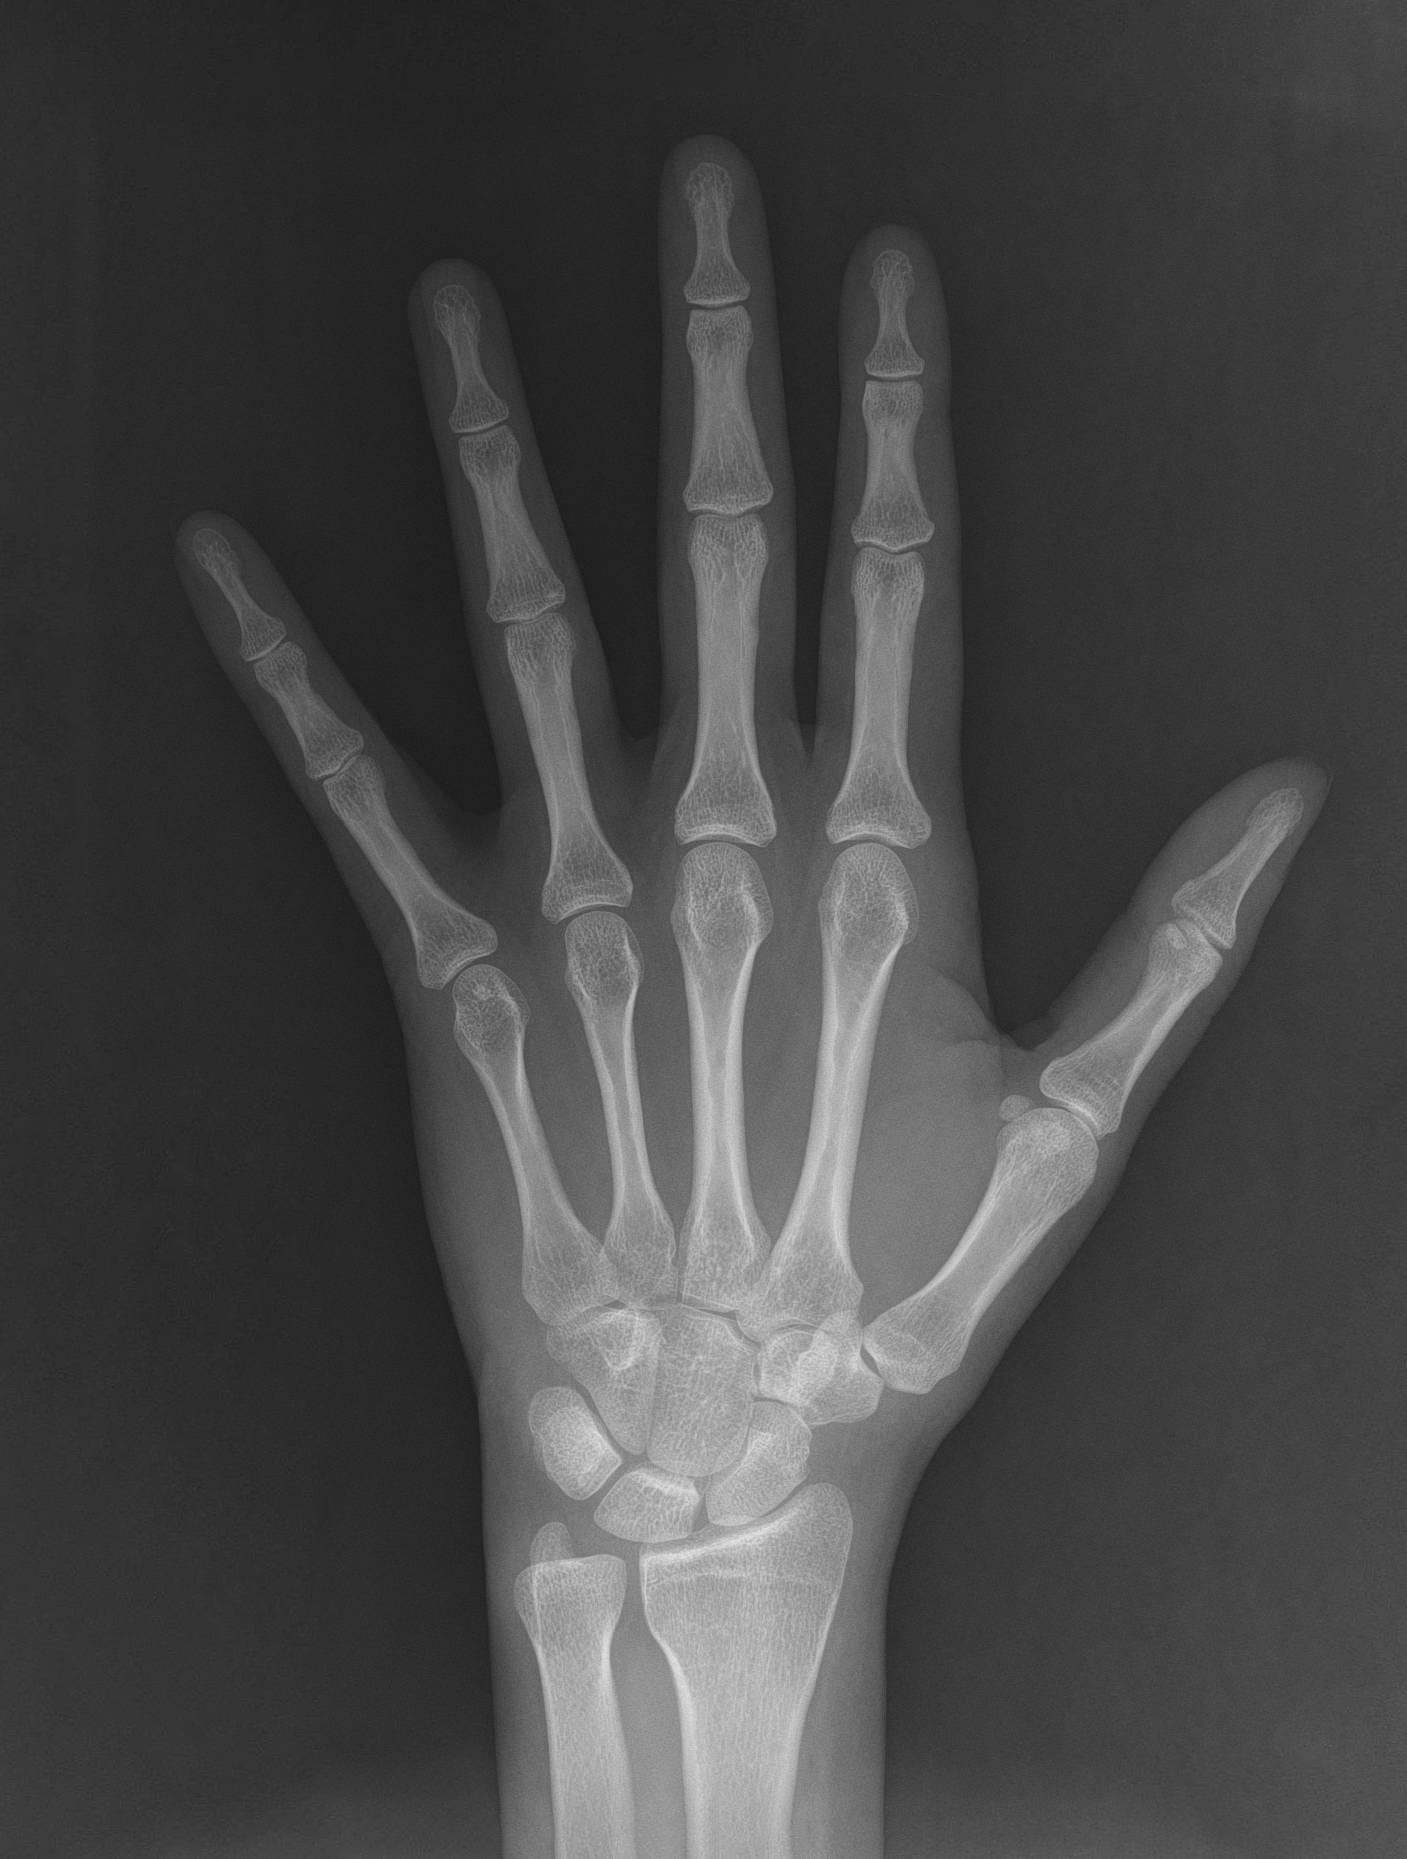
\includegraphics[height = 6cm]{images/UAB002-LH.jpg}
	\end{subfigure}
	~
	\begin{subfigure}[b]{.48\textwidth}
		\centering
		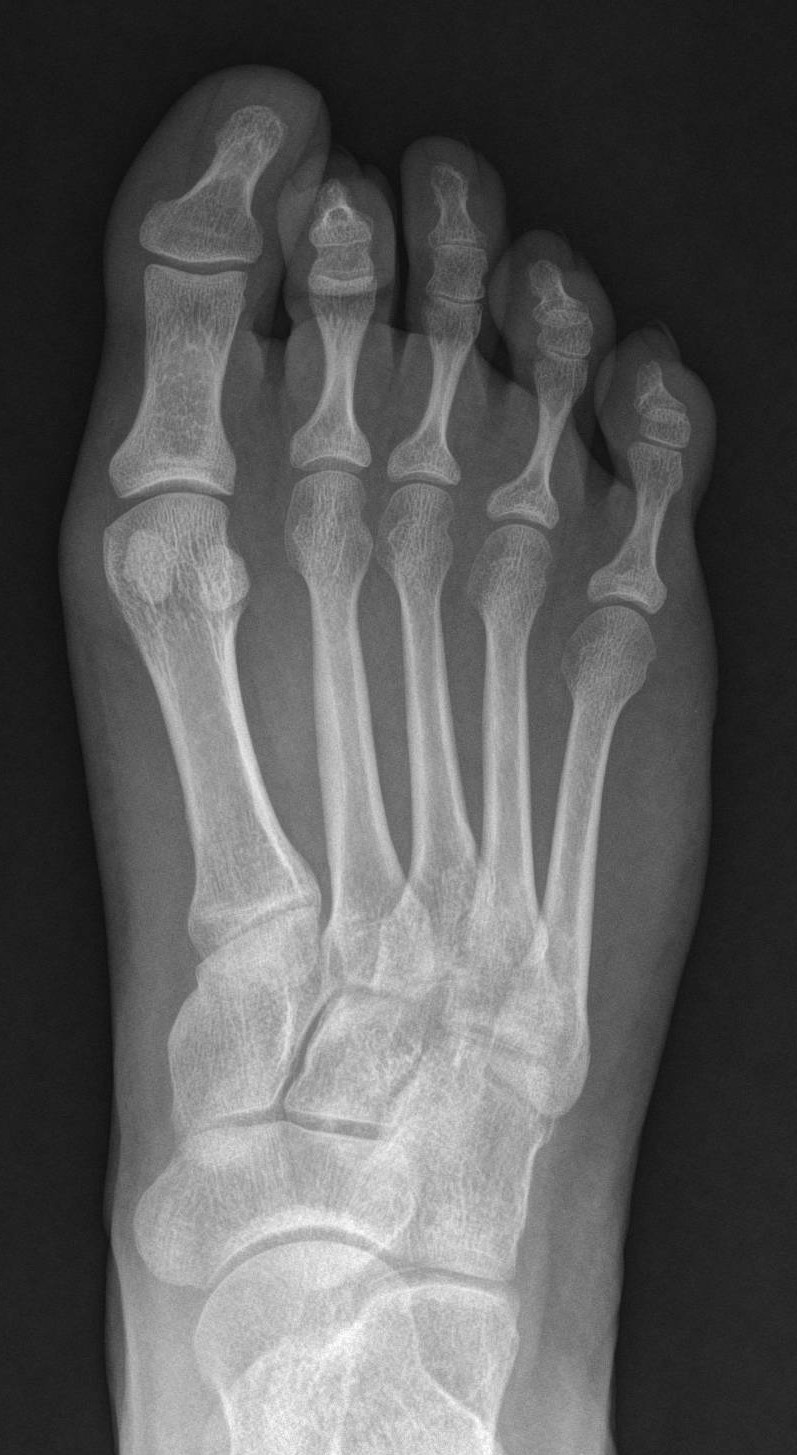
\includegraphics[height = 6cm]{images/UAB002-RF.jpg}
	\end{subfigure}
	
	\caption{Example images of a left hand and a right foot from the dataset.}
\end{figure}

\section{The Approach}

The task may be split into two parts---joint extraction and joint-by-joint assessment. In this work these tasks are being addressed by two different approaches and model architectures.

\subsection{Joint Extraction}

To extract joints from image, the Matterport implementation\cite{matterport_maskrcnn_2017} of Mask R-CNN was employed. The benefit of using a ready implementation is not only a labour elimination, but also pre-trained weights which may be used for transfer learning. This implementation also comes with several tools for data and model statistics visualization.

\subsubsection{Data Preparation}

Since the data don't include any joint location labels, they were annotated manually. To avoid the time-consuming and exhausting process of labeling the whole dataset, the labeling went iteratively: the first 80 images were randomly selected and labeled to be used for the model training. After that, the all images were fed to the model and according to the visual inspection of the model outputs additional images with certain features were included into the training set.

The four distinct models were proposed to extract joints---for feet, hands, wrist erosion regions and wrist narrowing regions. The feet detector extracts five metatarsophalangeal (MTP) joints and a toe proximal interphalangeal (PIP) joint; the hands detector extracts five PIP joints, five metacarpophalangeal (MCP) joints and a carpus region. The extracted carpus regions are then being fed to the two wrist models---feeding a carpus RoI instead of a whole image is intended to improve the detection accuracy.

So, the data preparation process goes in parallel with the model training and may be described this way:
\begin{enumerate}
	\item Select random 80 images
	\item Train a model on them
	\item Feed all images to the model
	\item Visually inspect the model outputs and if they are unsatisfying, add problematic images to the training set and go to step 2
\end{enumerate}
The hands detector model was used to obtain extracted carpus regions, which where later being prepared in similar way for training the wrist models. Totally the 168 images were annotated for the feet detector, 152 for the hand detector, 137 for wrist erosion and narrowing detectors.

An important step is the flipping the images of right or left limbs to obtain a dataset only of left or right limb images. This step eliminated most of joint misclassification issues and significantly increased a classification accuracy.

The all four data sets were augmented in the same way: 50\% chance of applying a Gaussian blur on 50\% of image area (some images in data set are blurry); linear contrast in range [0.75, 1.5] and multiplication in range [0.8, 1.2] (the data set images noticeably vary in contrast); [-5, 5] percent translation along both axis, [-20, 20] percent zoom and rotation in range [-15, 15] degrees.

The feet/hands images were resized to $512 \times 512$ size before being fed to the model; the wrist models inputs were $256 \times 256$. From each dataset its mean was extracted.

\subsubsection{Training and Results}

The Mask R-CNN implementation authors propose the two-step training---train the heads first and then (optionally) fine-tune the whole model including the backbone. In this work the fine-tuning wasn't performed, and the further text describes the heads-only training.

The models were trained with hyperparameters being mostly default. The important hyperparameters which were overridden are Batch Size = 8 and Detection Minimal Confidence = 0.0 (no region reject by the confidence score lower bound). The learning rate was set to 0.01 with exponential decay 0.98 per epoch for hands/feet models and 0.99 for wrist models---this allowed to accelerate the training with no significant negative effects in comparison with the default fixed learning rate 0.001. The implementation uses the SGD with momentum and gradient norm clipping (both left default).

All models were validated on 8 images. The best models were chosen by their class scores (except the wrist erosion detector)---the joint misclassification was considered the main issue at the joint extraction step. The wrist erosion detector was chosen by the overall validation loss value to obtain a model with a better bounding box prediction.

\begin{figure}[h]
	\centering
	
	\begin{subfigure}[b]{.48\textwidth}
		\centering
		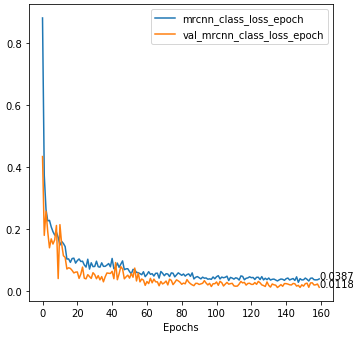
\includegraphics[height=6cm]{images/feet_model_class_loss.png}
	\end{subfigure}
	~
	\begin{subfigure}[b]{.48\textwidth}
		\centering
		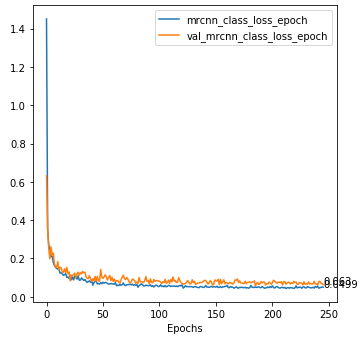
\includegraphics[height=6cm]{images/hands_model_class_loss.png}
	\end{subfigure}
	
	\begin{subfigure}[b]{.48\textwidth}
		\centering
		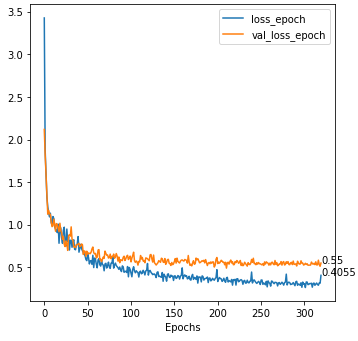
\includegraphics[height=6cm]{images/wrist_erosion_loss.png}
	\end{subfigure}
	~
	\begin{subfigure}[b]{.48\textwidth}
		\centering
		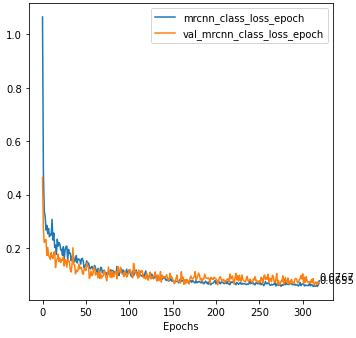
\includegraphics[height=6cm]{images/wrist_narrowing_class_loss.png}
	\end{subfigure}
	
	
	\caption{The selected training plots of the detection models. Note the absence of noticeable validation loss degradation during training.}
\end{figure}

The Mask R-CNN showed a fine accuracy both in terms of classification and bounding box regression. It was able to train itself on a relatively small amount of samples by training only its heads, and yield a very good result with a minimal count of misclassifications, which became a rare issue.

To further increase a joint detection accuracy, an additional step is being performed after a result is being obtained. If the model output doesn't contain a certain class, in most cases that means that a model still detected it but misclassified. The model output will have two or more instances of a certain class with different confidence score, and absent classes will be assigned to redundant instances with lower confidence scores.

\subsection{Damage Assessment}

Once the joint detection task is solved, it's now possible to actually assess the joint damage. The main fact around which the assessment model was built is a major label imbalance, which required some non-standard approach.

\subsubsection{Data Preparation}

The extracted joints were further split into three datasets---feet erosion scores, hands erosion scores and narrowing scores, according to the score scale. Each data set suffers a label imbalance and an extreme lack of samples for a certain class.

The train/validation data split was applied individually on each class to avoid some classes being completely absent in train or validation set. After the split, the most common class was undersampled to a count of the second most common class. The rest of classes the was oversampled.

The data augmentation consisted of [-10, +10] percent range zoom and shift, and rotation. The two rotation ranges were tested---30 and 45 degrees. The data were standardized sample-wise before feeding to a model. The two image sizes were tested---$128 \times 128$ and $64 \times 64$.

\subsubsection{The Model}

The DenseNet architecture was chosen to represent a joint damage estimator. The main reason was that the DenseNet has got a low parameter count, which coupled with the dense connectivity should provide a model robust against overfitting.

As the baseline, the Keras built-in DenseNet121 architecture was chosen, with some modifications:

\begin{itemize}
	\item The input $7 \times 7$ convolution with stride 2 was replaced by $3 \times 3$ convolution with stride 1. This was intended to prevent a too aggressive spatial sizes decrease, since input images were significantly smaller than traditional ImageNet $224 \times 224$.
	\item The last dense block was removed to simplify the model and decrease a free parameters count (from 7M to 4M).
	\item Specialized Dropouts\cite{specialized_dropouts} were implemented by the scheme $v_3$. The input data amounts will be low, so it's important to introduce external regularization.
\end{itemize}
Ultimately, the proposed estimator is a DenseNet88 model with a (6, 12, 24) dense blocks and a growth rate = 32. The rest of the model (except the final layer) remained the same, allowing to use the pre-trained ImageNet weights.

As an alternative, the custom architecture was built with the following differences:
\begin{itemize}
	\item The growth rate was reduced to 16
	\item The input $3 \times 3$ convolution was replaced by $7 \times 7$ convolution stride 1. The larger input convolution sizing was intended to increase the low-level feature extraction, which is important for this task.
	\item ReLUs were replaced by Leaky ReLU:
	\[
	\text{LReLU}(x) = 
	\begin{cases}
	\alpha x, & \text{if}\ x<0 \\
	x, & \text{if}\ x \geq 0
	\end{cases}
	\]
	where $0 < \alpha < 1$ is a hyperparameter, which was chosen as 0.2.
	\item The dense blocks were rearranged from (6, 12, 24) to (6, 12, 18).
\end{itemize}
This variant of a model provides only 0.8M of parameters and is intended to generalize better in case the first model will significantly overfit. This model variant won't be able to use built-in pre-trained weights, so it has to be pre-trained separately.

As an attempt to get around poorly represented labels, instead of classification the regression approach was chosen. Being significantly more complicated for deep learning models than classification, regression allows to overcome absence of samples for certain classes and still produce continuous output. Regression also takes label ordinality into account, so no artificial ordinality propagation is needed unlike the case of classification. To force the output stay in range, the sigmoid nonlinearity was used instead of linear, which is default for regression models. All outputs the network will produce will be in range $[0, 1]$, which allows to easily re-scale them to obtain SvH scores.

\subsubsection{Training and Results}

To maximise the model performance on small data, the 5-fold cross-validation was implemented. The models obtained were composed into ensemble by averaging their outputs.

The first model variant was initialized by ImageNet weights from DenseNet121. It was able to train itself only after forcing a high regularization---the higher dropout rate bound was set to 0.75 before the model started to train itself, and the best results were obtained with higher bound = 0.875. The $L^2$ regularization with $\lambda = 0.0001$ also showed itself beneficial for the training.

The best results were obtained by using the MAE as a loss function for erosion models and logcosh for the narrowing ensemble:

\begin{align}
\text{MAE}     &= \frac{1}{|\mathcal{X}|} \sum_{(x, y) \in \mathcal{X} } | x - y | \nonumber \\
\text{logcosh} &= \frac{1}{|\mathcal{X}|} \sum_{(x, y) \in \mathcal{X} } \log(\cosh(x - y)) \nonumber
\end{align}
where $\mathcal{X}$ denotes a batch. The models were trained using the Adam optimizer with a fixed learning rate 0.0001. The models were tested on input images resized to $64 \times 64$ witch batch size = 128.

The second model variant was tested after training from scratch and after initialization by pre-trained on CIFAR-10 weights. The higher dropout rate bound was reduced to 0.25, while the lambda for $L^2$ regularization remained 0.0001. The rest of hyperparameters remained the same, except the input and batch sizes---the erosion ensembles were trained on $128 \times 128$ with batch size = 32, while the narrowing models were trained on $64 \times 64$ images with batch size = 128. The model used to obtain CIFAR-pretrained weights was trained using similar hyperparameters, except the input size $32 \times 32$ and a batch size = 256. The pre-training lasted 50 epochs.

\begin{figure}
	\centering
	\begin{subfigure}[b]{.48\textwidth}
		\centering
		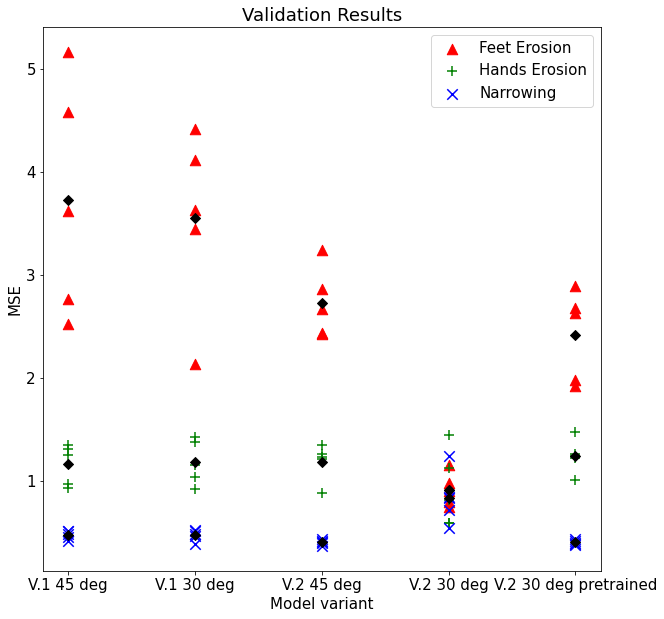
\includegraphics[height=6cm]{images/validation_results.png}
	\end{subfigure}
	~
	\begin{subfigure}[b]{.48\textwidth}
		\centering
		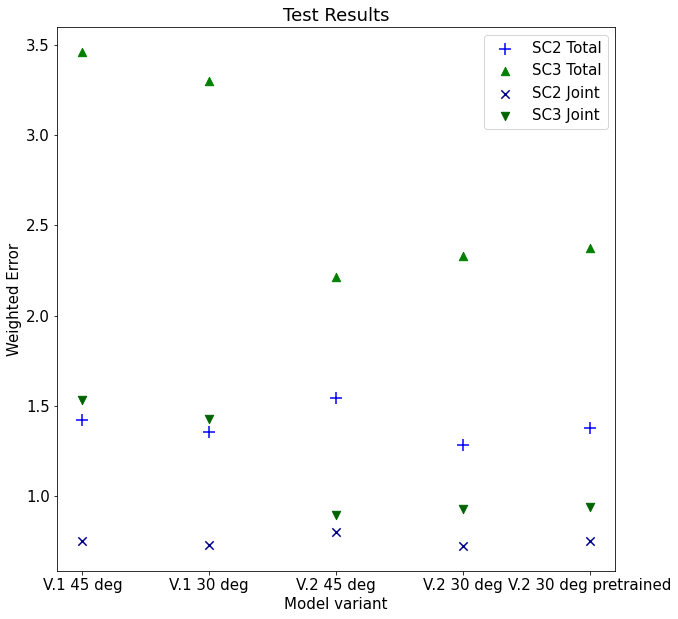
\includegraphics[height=6cm]{images/test_results.png}
	\end{subfigure}
	
	\caption{Left: validation results. Right: test results. The tested models include variant one and two trained with 30 and 45 degress image augmentation. The fifth model is a V.2 with 30-degree augmentation initialized with CIFAR-pretrained weights.}
\end{figure}

The best results vary for different models. The second proposed model showed a significant performance boost in terms of erosion assessment, while performing roughly the same while scoring the joint space narrowing. The best model overall may be considered the variant two trained on 30-degree augmentation from scratch---while showing slightly worse test performance than the 45-degree augmentation-trained one in terms of joint erosion, it performs noticeably better on the joint space narrowing assessment.

Since the model output layer is a sigmoid, it will never yield zero values for joints with no damage. Using the prior knowledge that most of joints assessed will have zero score, the output SvH scores lower than a certain threshold (0.5 was chosen) were overridden by 0.0 to allow a more precise overall scores computing. Without thresholding, the overall scores will be biased outwards zero due to the constant non-zero values of a joint-wise assessment.

\section{Discussion}

The algorithm above is the result of a trial-error approach. In this subsection the proposed approach details and hyperparameters choose will be discussed along with the results explanation.

\subsection{Joint Extraction}

\begin{itemize}
	
	\item \textbf{Object Detection instead of Semantic Segmentation}. The first approach for joint extraction was a semantic segmentation model (several U-Net variants). This approach showed unsatisfying results, primarily due to difficulties with producing a solid regions and a joint classification. Unlike semantic segmentation models, object detection architectures are designed for detecting individual and solid objects, considering groups of pixels instead of individual per-pixel classification.
	
	\item \textbf{Instance Segmentation instead of Object Detection}. While in this work masks had no use, the instance segmentation model is more beneficial due to using more of label accompanying information---the object mask brings more information about the object boundaries than a simple bounding box.
	
	\item \textbf{Partial model training}. Only the Mask R-CNN heads were trained, leaving the backbone untouched. The backbone training appeared to be significantly computationally heavy while bringing no benefits and letting the model to overfit. The training plots show that partial training is very robust to overfitting and the validation loss won't degrade as the training progresses.
	
	That may be explained by the fact that high-level layers (such as the model heads) are difficult to overfit, since they operate with an abstract information which is very similar for training and validation sets. The backbone is responsible for extracting low- and mid- level features, which may differ between sets and thus fitting the model for them will lead to information memorizing.
	
	\item \textbf{Low validation data amount}. 8 images were considered enough for validation since each image provides an information about the model loss relative to the bounding box regression, classification scores and mask predictions---i.e. providing much more information than could be expected from classification or semantic segmentation model. Coupled with the previous point about the overfitting robustness, this allows to feed more samples to the model with no concern about validation accuracy.
	
	\item \textbf{High initial Learning Rate}. The trainable part of a model is relatively shallow, which allows to use learning rates in order or two of magnitude higher than for the whole model. The training benefits from such a "quick start", while the LR decay gradually decreases learning rate to conventional values and allows to fit the data more precisely.
	
\end{itemize}

\subsection{Damage Assessment}

\begin{itemize}
	\item \textbf{Low-level feature engineering.} Despite the fact that deep learning models are able to train themselves on raw data, small datasets may significantly benefit from artificial construction of features more expressive than raw pixels. In this work, no feature engineering was performed, but the significant performance boost is expected if the proper feature construction method would be applied.
	
	\item \textbf{Data sampling}. Since the data show massive imbalance between labels, they have to be artificially balanced. The three approaches were tested---sample weights, naive oversampling and combined under- / over- sampling.
	
	The sample weights were computed to keep their sums across the certain class equal. E.g., if 1000 samples with a label A got a weight 0.001, 10 samples with label B will have their weights 0.1, while a single sample with a label C will have a weight 1.0. Weights are used to multiply the loss value of a model after applying on a certain sample.
	
	The class weight approach didn't significantly improved the model performance. The next employed approach was an oversampling---duplicating samples of more rare classes to obtain equal sample counts for all classes. This approach introduces a proper balancing, while copied samples will undergo data data augmentation which will differentiate then to a certain extent. The main drawback of the method is that it significantly inflates the data set size---if the first and second maximum label frequencies differ by $m$, at least $m(n-1)$ additional copies will be added to the dataset, where $n$ is a class count.
	
	\begin{figure}[h]
		\centering
		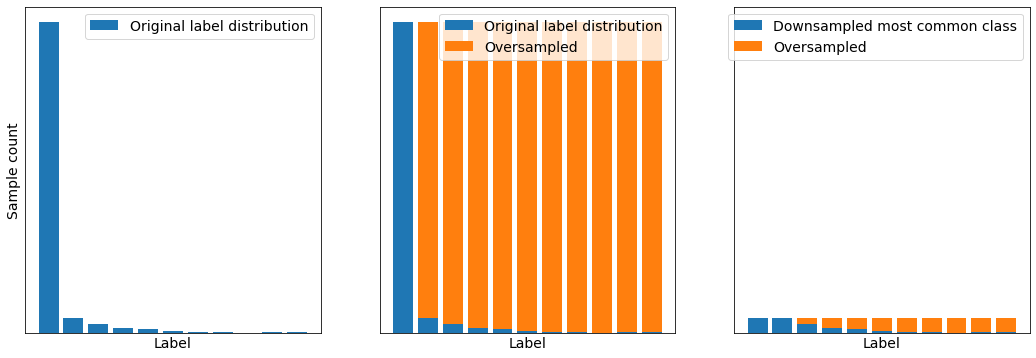
\includegraphics[width=\textwidth]{images/oversampling.png}
		\caption{Oversampling and combined approach illustrated.}
	\end{figure}
	
	To address the performance issue, the oversampling method was combined with the most common class undersampling. Only subset of the most common class was sampled from the data set, with the rest of data points oversampled. The most common labels in data sets are zeros, and zero-labeled samples introduce less features than any other, so no significant performance decrease is expected from zero data points undersampling. 
	
	\item \textbf{Sample-wise standardization over the dataset-wise}. The dataset-wise standardization (subtracting the dataset mean and scaling by the dataset standard deviation) showed itself numerically unstable due to the envoronment (Keras with Tensorflow backend) forcing to use float32 numbers. That led to the different statistics of train and validation sets and degraded the model performance.
	
	\item \textbf{Input Sizing}. Input sizing is important for the models since they were intended to be trained on the external computational cluster with a limited training time. While the first model variant provided more layers and parameters, its input size couldn't be increased within staying in time limits. The second model variant bypassed it by its significantly reduced size and an erosion assessment got a huge accuracy boost.
	
	\item \textbf{Augmentation}. The 45-degree rotation showed itself more destructible in comparison with 30-degree. Rotating an image too much makes it significantly differ from the validation/test set images, especially if the joint was already rotated on the original image (like thumb or hand minimus joints).
	
	The assessment accuracy is expected to be higher if all joint images would be oriented similarly, which would allow to not infer duplicating filters for differently oriented relevant features.
	
	\item \textbf{Erosion and Narrowing accuracy}. Erosion models (especially the feet erosion one) experienced unstable and highly variying results, while the JSN models showed training dynamics much closer to the ordinary training tasks.
	
	That may be explained by the fact, that erosion assessment includes much more complicated and high-level features---looking for bone damage requires looking for specks or pits, and requires an analyse of a surrounding context. At the same time, narrowing requires only distance measurement between two bones. Joint erosion model requires significantly larger training set to be properly trained and has to be more complex to fit data. JSN models also don't suffer performance loss after input images downsizing---narrowing still will be well-visible while erosion features occupy noticeably smaller image area.
	
	\item \textbf{Loss function choice}. A typical choice for regression models is MSE, which multiplies the model output gradient by the error size. It could be considered a proper choice for this task also, since the challenge test metric is a weighted RMSE. But the models showed best results using MAE and logcosh for erosion and narrowing respectively.
	
	\begin{figure}[h]
		\centering
		\begin{subfigure}[b]{.48\textwidth}
			\centering
			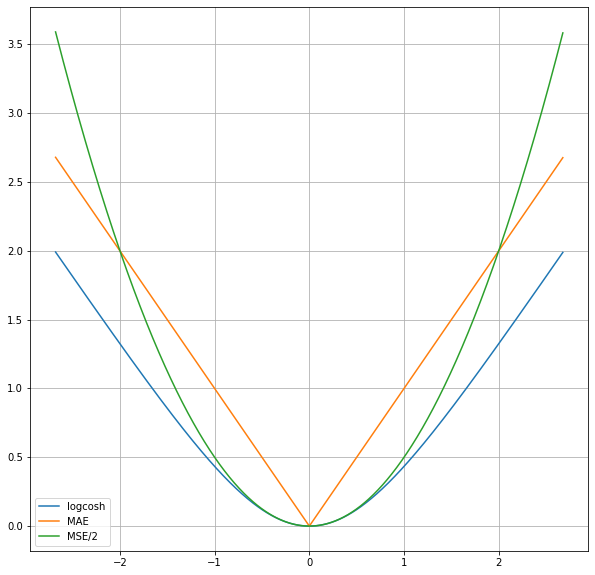
\includegraphics[height=5cm]{images/losses.png}
		\end{subfigure}
		~
		\begin{subfigure}[b]{.48\textwidth}
			\centering
			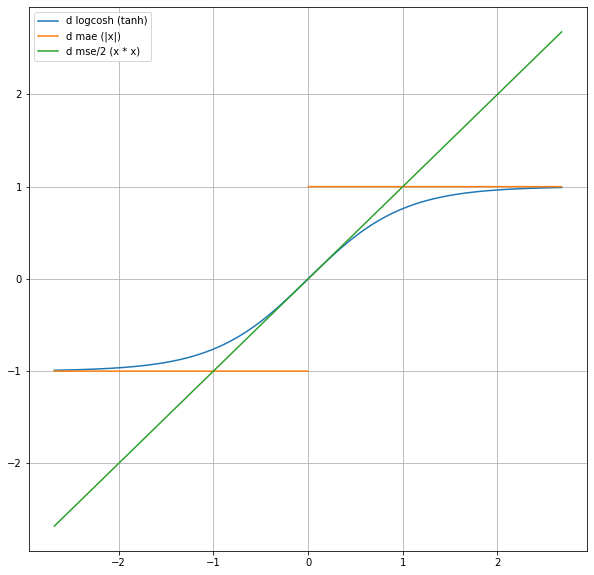
\includegraphics[height=5cm]{images/loss_derivatives.png}
		\end{subfigure}
		\caption{Left: different loss functions illustrated. Right: their derivatives.}
	\end{figure}
	
	The possible explanation may be an accessible data amount, which is too low for the proposed erosion models. MAE, while providing a constant loss-by-model-output derivative value, is more robust to outliers and noisy data, which the erosion data probably are. At the same time, the narrowing models benefit from logcosh or similar function since the narrowing data amounts are appropriate.
	
	Since the MAE loss may be too "rude" and yield a high update values, the Leaky ReLU was introduced to the second model variant to avoid the neuron death.
	\item \textbf{Fixed Learning Rate}. The learning rate is fixed since the annealing showed no positive result, sometimes even degrading the performance.
	
	The lower learning rate values degraded the performance due to the possible complex multi-level loss function landscape. Decreasing the learning rate  makes the loss value more sensible to smaller landscape details and allows to additionally decrease the training loss once it starts plateauing. In most tasks this allows to additionally improve validation results, but on small data sets this may lead to worse generalization, since loss and validation loss function relief details differ more significantly. The more data will be available, the more training and validation loss reliefs will be similar and the lower learning rates may be used without the issue.
	
	\item \textbf{Regularization}. The low data amount requires an external regularization in addition to the Batch Normalization and skip connections. While the $L^2$ regularization with $\lambda = 0.0001$ showed itself beneficial for both architectures, the first variant suffered a poor convergence with dropout rates lower than a certain lower bound. It started to generalise with maximal dropout rate $\geq 0.75$ and achieved the best performance with maximal dropout rate 0.85-0.875.
	
	The second architecture with the twice lower growth rate was designed to address primarily this issue. The lower redundant feature maps count allowed to reduce the maximal dropout rate to 0.25, which signalizes about a more proper model sizing.
	
	\item \textbf{Pre-training with no positive effect}. The pre-trained model showed a slight decrease in performance. The several possible explanations include the one similar with the previous point (training loss converges faster to small landscape details), or the wrong features inferred on unrelated data set.
	
\end{itemize}

\setsecnumdepth{part}
\chapter{Conclusion}

In the first chapter of the thesis the common machine and supervised learning methods were introduced. The Deep Learning, an important Machine Learning branch, was also presented with its peculiar properties. Finally, the key model family---the Convolutional Neural Networks---were described with their key principles, advantages and weaknesses. The chapter was finalized by some additional common Machine Learning techniques intended to help a certain model achieve a better result.

In the second chapter, the certain techniques which were employed to solve the task were portrayed---model architecture building methods, model architectures themselves and methods of further improving of their performance.

Finally, in the most important Practial Part chapter the actual experiments were described and their results were discussed with possible explanations and heuristics used to solve the task. Despite the difficulties with the low data amounts, the proposed method showed itself as an able to produce meaningful results.

Limited data amounts are a common issue in a healthcare, but the overall accessible data growth takes place in medical imaging also. The growing data sets would allow to shift the focus from designing models for small data to designing systems which fully utilize the power of big data sets and Deep Learning methods. The tendency of providing more open data along with rapid progress in the Deep Learning allow to look at the possibility of learnable models adoption in healthcare with optimism.

For the further work on related tasks, it may be beneficial to couple the deep learning methods with low-level feature construction. While the Deep Learning models are designed to be applied on large amounts of raw data, their flexibility may allow to use them in different way, like fitting smaller amounts of well-expressed data. Another proper improvement that could be done over the proposed method is a construction of a monolithic model, able to train itself end-to-end.

\bibliographystyle{iso690}
\bibliography{mybibliographyfile}

\setsecnumdepth{all}
\appendix

\chapter{Acronyms}

\begin{description}
	\item[ANN] Artificial Neural Network
	\item [BN] Batch Normalization
	\item[CNN] Convolutional Neural Network
	\item[CV] Computer Vision
	\item [FFNN] Feedforward Neural Network
	\item[JSN] Joint Space Narrowing
	\item [LR] Learning Rate
	\item[ML] Machine Learning
	\item[MAE] Mean Absolute Error
	\item[MCP] Metacarpophalangeal (Joint)
	\item[MSE] Mean Squared Error
	\item[MTP] Metatarsophalangeal (Joint)
	\item[NAG] Nesterov Accelerated Gradient (Descent)
	\item[PIP] Proximal Interphalangeal (Joint)
	\item[RA] Rheumatoid Arthritis
	\item[ReLU] Rectified Linear Unit
	\item[RMSE] Root Mean Squared Error
	\item [RoI] Region of Interest
	\item [RPN] Region Proposal Network
	\item [SGD] Stochastic Gradient Descent
	\item[SvH] Sharp/van der Heide method
\end{description}

\chapter{Example Training Plot}

\begin{figure}
	\centering
	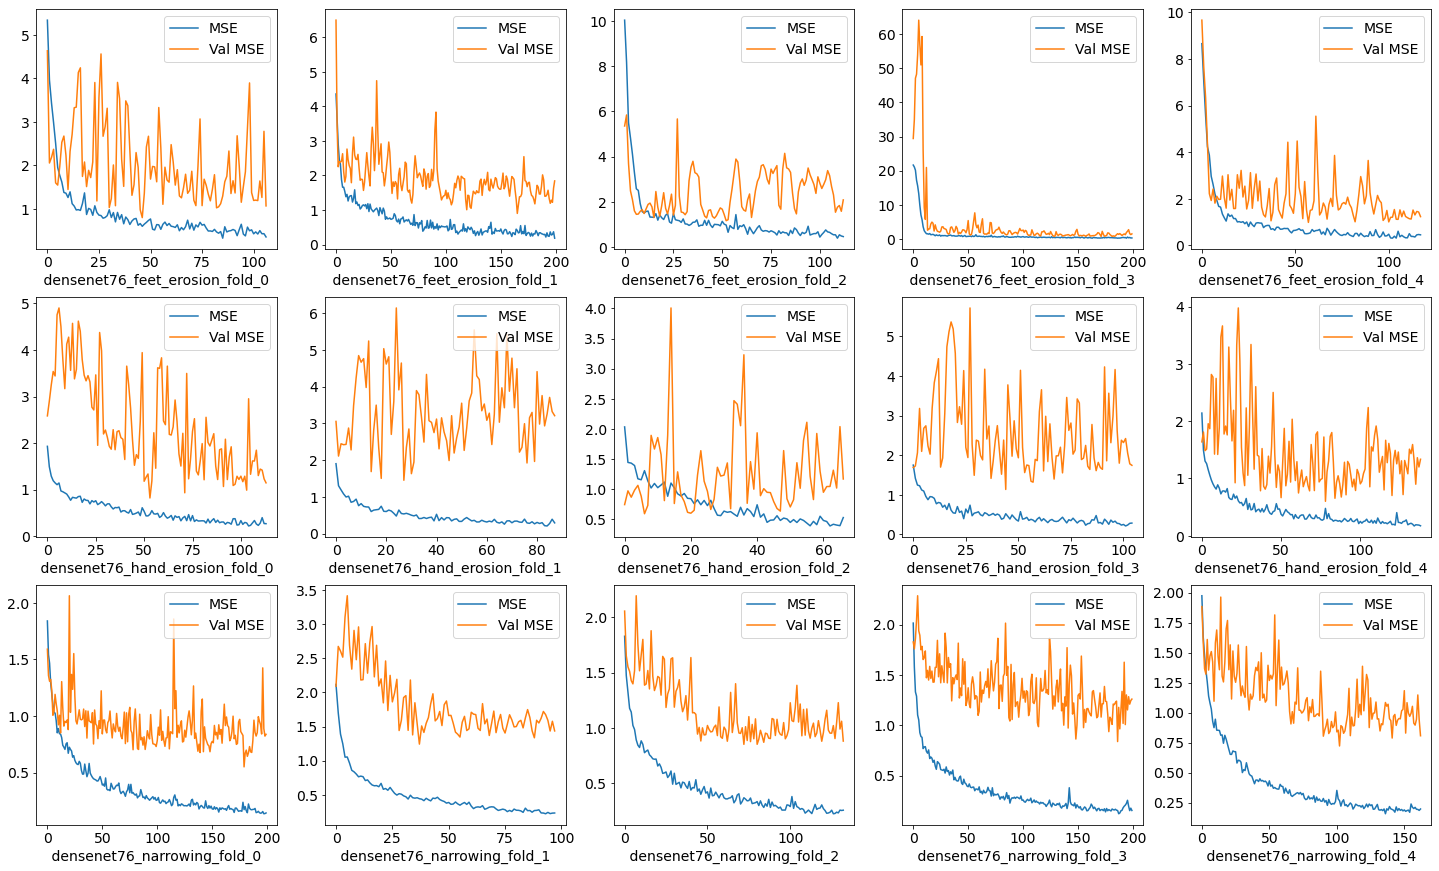
\includegraphics[angle=90, width=\textwidth]{images/results.png}
	\caption{Training plot for a second model variant trained from scratch on 30-degree augmented images}
\end{figure}

\chapter{Contents of enclosed CD}

The sources also will be available at \url{https://github.com/EternalSorrrow/bak}.

\begin{figure}
	\dirtree{%
		.1 readme.txt\DTcomment{the file with CD contents description}.
		.1 notebooks\DTcomment{the directory with Colab notebooks used for work}.
		.2 ra2\textunderscore feet\textunderscore joint\textunderscore detection.ipynb\DTcomment{the notebook for feet joint model}.
		.2 ra2\textunderscore hands\textunderscore joint\textunderscore detection.ipynb\DTcomment{the notebook for hands joint model}.
		.2 ra2\textunderscore wrist\textunderscore erosion\textunderscore joint\textunderscore detection.ipynb\DTcomment{the notebook for wrist erosion regions}.
		.2 ra2\textunderscore wrist\textunderscore narrowing\textunderscore joint\textunderscore detection.ipynb\DTcomment{the notebook for wrist narrowing regions}.
		.2 ra2\textunderscore docker\textunderscore test.ipynb\DTcomment{the notebook used for the model training on Colab}.
		.1 BP\DTcomment{the directory of \LaTeX{} source codes of the thesis}.
		.2 BP\textunderscore Yorsh\textunderscore Uladzislau\textunderscore 2020.pdf\DTcomment{the thesis text in PDF format}.
		.2 BP\textunderscore Yorsh\textunderscore Uladzislau\textunderscore 2020.tex\DTcomment{the thesis text .tex source}.
		.2 images\DTcomment{directory with the images used in the thesis}.
		.1 docker\DTcomment{the docker sources directory}.
		.2 Dockerfile\DTcomment{the dockerfile for the project}.
		.2 run.sh\DTcomment{the executable container script}.
		.2 script.py\DTcomment{the .py script which trains the models and produces an output}.
		.2 test.py\DTcomment{test .py script used to test the GPU visibility}.
		.2 weights\DTcomment{the directory with pre-trained weights}.
		.3 weights.h5\DTcomment{the CIFAR-pretrained weights for DenseNet76 (second model variant)}.
		.2 trained\textunderscore models\DTcomment{the pre-trained detectors directory}.
		.3 mrcnn\textunderscore feet\textunderscore mrcnn\textunderscore class\textunderscore loss\textunderscore best-160.hdf5\DTcomment{a pre-trained feet joints detector}.
		.3 mrcnn\textunderscore hand\textunderscore mrcnn\textunderscore class\textunderscore loss\textunderscore best-200.hdf5\DTcomment{a pre-trained hand joints detector}.
		.3 mrcnn\textunderscore we\textunderscore loss\textunderscore best-320.hdf5\DTcomment{a pre-trained wrist erosion regions detector}.
		.3 mrcnn\textunderscore wn\textunderscore mrcnn\textunderscore class\textunderscore loss\textunderscore best-320.hdf5\DTcomment{a pre-trained feet joints detector}.
	}
\end{figure}

\end{document}